% PAIEC 2026 technical report, version 2. Build: make pdf (pdflatex + bibtex; see Makefile). Continues bericht/paiec_report.tex.
% Every number in this file points to a file/field in ZAHLEN-QUELLEN-v2.md and is checked by pruefe_zahlen.py before each build.
\documentclass{article}

% Workshop option with single-blind reviewing = author names visible (competition: reports need not be anonymous).
\usepackage[sglblindworkshop,final]{neurips_2026}
\workshoptitle{Predictive AI Evaluation Competition (PAIEC)}

\usepackage[utf8]{inputenc}
\usepackage[T1]{fontenc}
\usepackage{hyperref}
\usepackage{url}
\usepackage{booktabs}
\usepackage{array}
\usepackage{placeins}
\usepackage{longtable}
\usepackage{amsfonts}
\usepackage{amsmath}
\usepackage{nicefrac}
\usepackage{microtype}
\usepackage{xcolor}
\usepackage{graphicx}
\usepackage{float}
\graphicspath{{abbildungen/}}
\hypersetup{hidelinks,pdftitle={When is an AI system's response to a benchmark item predictable, when is it not, and what sets the error?},pdfauthor={Christian Bucher}}

\newcommand{\BB}{\textsc{bb}}
\newcommand{\EM}{\textsc{em}}
\newcommand{\dd}{-{}-}% two hyphens in commands, never an en dash
% --- submission package (switch here if the package changes; pruefe_zahlen.py checks the hash against the file) ---
\newcommand{\pkgfile}{paiec\_v2core\_final.zip}
\newcommand{\pkghash}{3274b09524221ac268be41f8b52fc56ca341daf72cf9734561be00e0f3a1e331}
\newcommand{\pkghashshort}{3274b095}
\newcommand{\pkghashtex}{3274b09524221ac268be41f8b52fc56c\allowbreak a341daf72cf9734561be00e0f3a1e331}
\newcommand{\pkgbytes}{32,379}
\newcommand{\pkgstate}{3c46e5bd4496d360}
\newcommand{\repourl}{{\small\urlstyle{same}\url{https://github.com/christian140903-sudo/christian140903-sudo/tree/claude/technosignatures-archive-analysis-nxoino/paiec-2026}}}
\newcommand{\repotag}{v2.0.1-paiec}
\newcommand{\prereghash}{e5fd821fdf6e2db3be86e1e341b02bc4199d4721790dd3ae8f027b60e9521ab7}
\newcommand{\prereghashshort}{e5fd821f}
\newcommand{\prereghashtex}{e5fd821fdf6e2db3be86e1e341b02bc4\allowbreak 199d4721790dd3ae8f027b60e9521ab7}
\newcommand{\preregtime}{2026-10-20 20:26:04 UTC}
% --- end-of-main-text marker: page and vertical position are written to \jobname.mainend at shipout (read by pruefe_zahlen.py) ---
\newwrite\mainendfile
\immediate\openout\mainendfile=\jobname.mainend\relax
\newcommand{\markmainend}{\pdfsavepos\write\mainendfile{\thepage\space\the\pdflastypos\space\the\paperheight}}

\title{When is an AI system's response to a benchmark item predictable, when is it not, and what sets the error?\\
\large A decomposition, bounds and a method league for the Brier learning curve under the PAIEC protocol, with a
confirmatory re-analysis on fresh seeds and an audit of the training release}

\author{%
  Christian Bucher\\
  Independent researcher\\
  Vienna, Austria\\
  \texttt{christian140903@gmail.com}
}

\begin{document}

\maketitle

\begin{abstract}
When can the correctness of an AI system's answer to a benchmark item be predicted, and what sets the error? We study
this for the PAIEC protocol (Brier learning curve over 0--31 revealed labels per subject--benchmark pair) on 142 public
benchmarks held out benchmark-wise, with a text-free hierarchical predictor as the submitted model and a confirmatory
re-analysis on fresh seeds with rules frozen before the runs. (i) An exact three-term learning
curve (prior, sampling, split) with all moments taken from the data and nothing fitted matches the beta-binomial
baseline within 5\% at every budget on fresh seeds (Design B; rule: $\pm 10\%$); our stated expectation of $\le 3\%$ was
missed at budget 31. (ii) Bounds locate the reachable gains: a pair-level floor for text-free predictors, a
benchmark-location oracle at budget 0, and a per-benchmark response-noise floor with median 0.049 (IQR 0.011--0.088) on
the 62 benchmarks with at least 100 repeated cells. (iii) In the confirmatory runs (benchmark-cold Design A and
subject-cold Design B) nine of ten frozen hypotheses passed and one failed (H4, below). With one subject per benchmark the submitted
predictor is neither shown better than nor equivalent to the beta-binomial baseline (\mbox{$-0.0004 \pm 0.0004$} ALC in both
designs, grey zone); with three subjects sharing the labels it is better by \mbox{$0.0049 \pm 0.0007$} (both designs). Subject
identity shows a small effect (2.1--2.6 SE); the equivalence hypothesis failed. In a method league over all 10 folds,
with one subject per benchmark none of the smoothing, IRT, matrix-factorisation, kNN or stacking families is
distinguishable from the submitted model; gradient boosting and the unsmoothed baselines are worse, and from two subjects
on the submitted model is best or tied-best in every regime. (iv) An audit of the training release (9 findings, 17 evidence packs, 3 patches) accompanies the submission.
Code and report: \repourl{}.
\end{abstract}

\section{Introduction}
\label{sec:intro}

When is an AI system's response to a benchmark item predictable, when is it not, and what sets the error? Our thesis is
that, under the PAIEC protocol and for predictors that use no item text, the error is \emph{information-limited, not
model-limited}: it is set by what the protocol reveals (labels, subjects of the same benchmark sharing them, the item
split, the item count), not by the choice among estimators that use the revealed labels. We test this; we do not assume it.
Item response models evaluate language models on fewer items \citep{polo2024tiny, kipnis2024metabench,
vivek2023anchor}, capability measures predict performance across models \citep{ruan2024observational,
owen2024predictable}, and amortised, text-based item parameters are the organisers' own line
\citep{truong2025amortized}; missing, to our knowledge, is what a label-budget protocol lets \emph{any} text-free
predictor achieve, how fast the remaining error falls with labels, and where it fails. PAIEC \citep{paiec2026} scores the Brier score \citep{brier1950} over subject--benchmark pairs as an area under
the learning curve (ALC) over budgets 0, 1, 3, 7, 15, 31 \citep{guyon2011alc}, on benchmarks disjoint from training.

\textbf{Contributions.} (a) An exact per-pair decomposition and a ladder of oracle bounds down to the per-benchmark
response-noise floor (\S\ref{sec:theory}). (b) A three-term learning curve for posterior-mean predictors derived from
the protocol, tested with no fitted parameter on fresh seeds, and its measured limit, pooling. (c) Protocol dependence as
tested statements (Table~\ref{tab:protocol}). (d) A method league under one protocol and a hypothesis table reported as
it fell, including a failed hypothesis. (e) A data-quality audit of the training release with evidence packs, patches, a
curation metric and a checking tool (\S\ref{sec:audit}).

\begin{figure}[t]
  \centering
  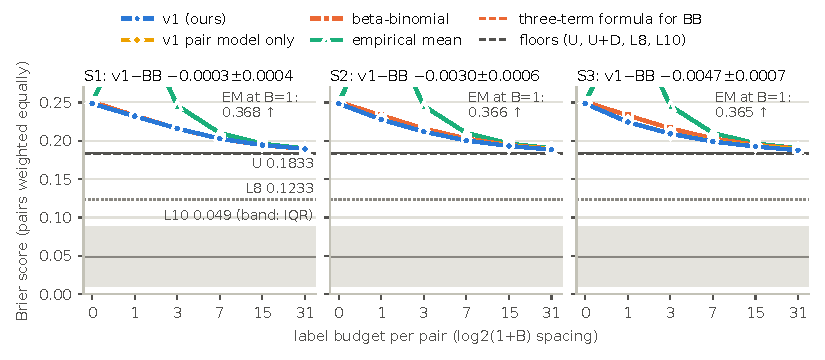
\includegraphics[width=\linewidth]{fig1_lernkurven.pdf}
  \caption{The map (discovery set): Brier per budget for \EM, \BB, the pair-level model and the submitted model at one,
  two and three subjects per benchmark, with the pair-level floor $U$ and the three-term curve for \BB\ (dashed, nothing
  fitted). Panel titles: submitted $-$ \BB\ $\pm$ SE (``v1'' in the panels = the submitted predictor along the v1 path, Appendix~\ref{app:prereg}). Grey: floor $U$ (thin: $U + D$), oracle L8, repeat-noise floor L10
  (median, band = IQR). Data: Table~\ref{tab:figsources}.}
  \label{fig:map}
\end{figure}

\section{Task, protocol and data}
\label{sec:data}

At each budget the platform calls \texttt{predict(input, labeled)} per distinct \texttt{[subject, item]}; the subject
is eight visible string fields, the benchmark an anonymous stable \texttt{benchmark\_id}. Per pair with $\ge 80$ items
the items are split 50/50 into acquisition and evaluation pools; labels are revealed at random, one recorded response
per item, nested over $B \in \{0,1,3,7,15,31\}$; the pair score is the Brier score over all recorded responses of its
evaluation items, and $\mathrm{ALC} = 0.1\,B_0 + 0.2\,(B_1 + B_3 + B_7 + B_{15}) + 0.1\,B_{31}$. The streaming driver
\citep{paiecbase2026} passes one \texttt{labeled} set per checkpoint to all targets of a run. A subject \emph{is}
its field dictionary: pairs with identical fields are indistinguishable, and every predictor, the organisers' baselines
included, counts their labels together ($\approx 2\%$ of pair--budget rows get more ``own'' labels than $B$; mean surplus
at $B = 31$: $+0.6$, $+1.2$, $+8.9$ with two, three, thirty subjects per benchmark, none with one). How many subjects
of one benchmark share a run on the platform is not public.

The only training source is the Measurement Data Bank \citep{mdb2026}, revision \texttt{54074453}: 156 public binary
benchmarks with grades, 31,389,917 subject--item rows, 68,268,267 responses; no other data, no text, no language model.
Responses are used as released (7 \texttt{lower\_is\_better} benchmarks unflipped); two groups are excluded on the
basis of the audit (\S\ref{sec:audit}): 64 bird\_sql configurations graded 0 on all 360 questions and 12 swebench\_live
subjects with only successes. Pairs with $\ge 80$ items occur in 142 benchmarks (12,918 pairs, median benchmark 13, two
benchmarks hold 59\%); 52\% of the pairs have no \texttt{normalized\_name}.

\section{Theory: what sets the error}
\label{sec:theory}

\textbf{Exact decomposition.} If a pair has success rate $R$ on its evaluation responses and a predictor issues
probabilities $q_i$ with response-weighted mean $\bar q$ (Appendix~\ref{app:theory}, A.1),
\begin{equation}
  \mathrm{Brier}_B = (\bar q - R)^2 + R(1-R) + G_B,
  \label{eq:brier}
\end{equation}
with item gain $G_B \le 0$ non-zero only with item-level information. $R(1-R)$ is the floor of every pair-constant
predictor; its ALC-weighted mean on the test pairs is $U = 0.1833$. Its Murphy decomposition
\citep{murphy1973partition, gneiting2007proper} shows for the submitted model (binned, $S = 3$) reliability $\le 0.0006$
at every budget and resolution 0.0022 of $\mathrm{Var}(R) = 0.0667$ at budget 0: budget 0 is a resolution problem, not a
calibration problem.

\textbf{Learning curve of a posterior-mean predictor.} For $q_B = (k + \kappa\mu)/(B + \kappa)$ with fixed prior
strength $\kappa$ ($\alpha + \beta$ of a Beta prior), $N$ items per pair split into halves $A$ and $E$, Appendix
A.2 derives in eight steps
\begin{equation}
  \mathrm{E}(q_B - R_E)^2 = \frac{B\,(U - (B-1)F) + \kappa^2 V_0}{(B+\kappa)^2} + \frac{B}{B+\kappa}\,D ,
  \qquad \mathrm{E}(q_0 - R_E)^2 = V_0 ,
  \label{eq:curve}
\end{equation}
with prior error $V_0 = \mathrm{E}(\mu - R_E)^2$, split term $D = \mathrm{E}[4\,\mathrm{Var}_i(p_i)/(N-1)]$ (the
acquisition half is not the evaluation half) and finite-population term $F = \mathrm{E}[\mathrm{Var}_i(p_i)/(N_A-1)]$.
It is the standard Bayesian mean-squared error of a posterior-mean predictor \citep{morris1983peb, efron1975stein},
applied to the competition protocol with a split term; $U, V_0, \kappa, D, F$ are moments of the data, not fitted
(discovery: 0.1833, 0.0673, 2.73, 0.00138, 0.00070; $N$ median 1,000, minimum 80). Disclosure: the split term was added
after a 13\% shortfall at budget 31 on the discovery set, before any confirmatory run (A.2). Consequences: $\kappa^* = U/V_0$ minimises every budget's error of the two-term form (2.76 with the split term; for a well-specified Beta prior
$U/V_0 = \kappa$ identically, so ``$\kappa^* \approx \kappa_{\mathrm{ML}}$'' is a specification test); the
$1/(B+\kappa)^2$ shape puts the loss early (budget 31 carries about 2\%); even a perfect prior leaves a pair-level floor
for text-free predictors of $U + \text{sampling} + \text{split} = 0.1948$ ALC, and the sampling term alone (0.0107)
exceeds the whole model--baseline gap at three subjects (0.0047).

\textbf{Validity limit: pooling.} The submitted model is \emph{not} a fixed-$\kappa$ predictor: its benchmark location
is updated from the other subjects' labels, so its effective $V_0$ depends on $S$ and $B$. With its own budget-0 excess,
Eq.~\ref{eq:curve} overstates its error at one label by $+17.6\%$ (three subjects) and $+78.4\%$ (thirty) on the
discovery set, vanishing by budget 31. We therefore describe pooling as a budget- and subject-count-dependent reduction
of the prior error, $V_0(S,B)$, and test it as H2b; the formula is not a general statement about learning curves. The identity
collision makes $S = 1$ the clean test regime.

\textbf{Bound ladder and noise floor} (Fig.~\ref{fig:ladder} in Appendix~\ref{app:tables}; A.5). At budget 0 the constant scores 0.2500, the
submitted model 0.2485, and a leave-one-out oracle of the benchmark location 0.2067: benchmark location is the largest
lever at budget 0 (65\% of $\mathrm{Var}(R)$), out of reach for text-free predictors under our rules (ability alone adds 3--6\%). The pair-rate
oracle gives $U = 0.1833$: the within-pair term is 73\% of the constant predictor's Brier score of 0.25 (92\% of
$\mathrm{Var}(y) = 0.199$); rate plus leave-one-out item difficulty removes a third of it ($0.1833 \to 0.1233$), and the cell-rate oracle $k/n$ leaves 0.0065 (L9, biased low: cells with one response contribute 0). The bottom is response noise: for cells with $n \ge 2$ responses,
$k(n-k)/(n(n-1))$ is unbiased for $p(1-p)$ (L10). On the 62 benchmarks with repeated responses the per-benchmark noise
floor has median 0.049 (IQR 0.011--0.088); the answer-weighted mean 0.044 is dominated by one benchmark, and L10 is a
subset bound because repeats exist only where curators recorded trials \citep[cf.][]{madaan2024variance,
miller2024errorbars, northcutt2021pervasive, gema2024mmlu}.

\section{Method}
\label{sec:method}

The submitted predictor models $\mathrm{logit}\, r_{sb} = c_b + a_b m_s + v_{sb}$ with $c_b \sim \mathcal{N}(\mu_c,
\tau_c^2)$, $a_b \sim \mathcal{N}(\lambda, \tau_\lambda^2)$, $v_{sb} \sim \mathcal{N}(0, s_s^2)$: $m_s$ is the subject's
ability from training (a ridge regression on visible metadata for unseen names); location $c_b$ and slope $a_b$ are
always cold, learned only from the labels of the run. Hyperparameters come from Gaussian marginal likelihood on inner
benchmark folds \citep{mackay1992evidence}. At test time the labels are filtered by \texttt{benchmark\_id} and grouped
by the eight fields; the posterior over $(c_b, a_b, v_1 \dots v_G)$ is a Laplace approximation solved in $O(G)$, the
probability its probit-approximated mean. An item stage adds a Laplace posterior for an item offset $d_i \sim
\mathcal{N}(0, \tau_i^2)$ from other subjects' labels on the same item ($\tau_i^2 = 2.55$ from a one-parameter IRT fit
\citep{lord1980irt, lalor2016irt}); without such labels it returns the pair-level value exactly. Platt scaling
\citep{platt1999probabilistic} per label stage is kept at stages 0 and 1 ($0.2527 \to 0.2485$ at budget 0; stage
choice in Section~\ref{sec:limits}). One file, standard library only, no network; \texttt{predict} never raises: on an
exception it falls back to a beta-binomial estimate from the pair's own labels, then to 0.5 (Appendix~\ref{app:protocol}).

\textbf{Why no text: a decision with a bound.} At budget 0 the submitted model scores 0.2485 and text-free ability oracles 0.2480--0.2460 (A.5); the benchmark-level oracle shows that benchmark-level text could lower this to at most 0.2067, and the item-difficulty oracle
puts the ceiling of item information at $-0.054$ ALC. That room is what amortised, text-based approaches target
\citep{truong2025amortized, zhou2025adele, pacchiardi2024hundred}; ours is complementary: it states what no text-free
predictor can do and how fast the remaining error falls with labels. A text-based item prior was prepared but not completed before the freeze and is not part of the submission
(Appendix~\ref{app:explore}).

\section{Experimental design}
\label{sec:design}

\textbf{Replica.} The offline evaluation re-implements the published protocol from the competition text and
\texttt{streaming\_ingestion.py} (read, not executed): 50/50 split per pair and seed, revealed labels as the first $B$
items of a random permutation of the acquisition half (equal in distribution to the platform's selection sampling), one
recorded response per revealed item, exact Brier over the evaluation items (assumptions A1--A5 and the leak regression:
Appendix~\ref{app:protocol}). We reproduce the organisers' Empirical Mean (\EM) and the beta-binomial baseline (\BB)
exactly in our harness (max $|\Delta q| = 0$).

\textbf{Designs, regimes, seeds.} Design A (benchmark-cold): 10 folds over 142 benchmarks, everything fitted on training
benchmarks only. Design B (benchmark- and subject-cold): names additionally split into 5 folds and removed from
training. At most 30 test pairs per benchmark (2,142 pairs). Regimes $S = 1, 2, 3$ with equal standing, $S = 30$ as a
limit, compact10 (10 subjects share 100 items) as a hypothetical bound for item overlap. The \emph{discovery set}
(fold seed 1234, seeds 0--2) is where every hypothesis in Table~\ref{tab:hyp} originated. The \emph{confirmatory
re-analysis} (fold seed 200, seeds 200--202) ran with rules frozen before the runs: the plan was fixed at
\preregtime{} (sha256 \texttt{\prereghashshort\ldots}; full hash and text in Appendix~\ref{app:prereg}), before the
first confirmatory run started, for the hardened variant of the submitted predictor (deviation noted in
Appendix~\ref{app:prereg}). It is confirmatory with respect to sampling randomness, not with respect to the
benchmark population: all hypotheses originated from the same 142 benchmarks.

\textbf{Decision rule.} All comparisons are paired over the same pairs and seeds, SE cluster-robust over benchmarks
\citep{cameron2015cluster}. \emph{Better}: $\hat d + 2\,\mathrm{SE} < 0$; \emph{worse}: $\hat d - 2\,\mathrm{SE} > 0$;
\emph{equivalent}: $|\hat d| + 2\,\mathrm{SE} < 0.001$ ALC (margin fixed in advance); otherwise \emph{grey zone}. Under
a null effect a false \emph{better} or a false \emph{worse} verdict each occur with probability 2.3\% (4.6\% for either);
equivalence is undecidable at $\mathrm{SE} \ge 0.0005$ and has 38\% power at $\mathrm{SE} = 0.0004$ (45--46\% at the
SE of 0.00038 observed for H1 at $S = 1$), so a grey zone there is ``not decidable''. About 20 directional verdicts are produced, so about 0.9 false ones are expected
under a global null (the pre-registration stated $\approx 0.5$, counting one direction only); no correction applied
(Appendix~\ref{app:prereg}); league competitors are tuned only on the training benchmarks of their fold.

\section{Results}
\label{sec:results}

% erzeugt von tabellen_v2.py aus JSON/CSV — nicht von Hand aendern
\begin{table}[t]
\centering\footnotesize
\caption{\raggedright Main result per regime. Columns 2--7: \textbf{discovery} (Design A, seeds 0--2, 10 benchmark folds, 2,142 test pairs, 142 benchmarks;
paired differences $\pm$ cluster-robust SE over benchmarks; letters = verdict by the rule of Section 5: b better, w worse, e equivalent, g grey zone).
Last two columns: \textbf{confirmatory} runs (seeds 200--202, fold seed 200; H1 of Table~\ref{tab:hyp}), Design A (benchmark-cold, all
regimes) and Design B (benchmark- and subject-cold, S1 and S3). ``ours'' = the submitted predictor; discovery numbers were computed along the v1
path, which differs from the submitted v2.0-core only in the Platt stages 3 and 7 (Appendix~\ref{app:prereg}). Sources: \texttt{modell/ergebnisse/cv\_A\_p2\_S1-S2-S3-S30-kompakt10/auswertung.json},
\texttt{liga/ergebnisse/liga\_vergleich.json} (ALC columns), \texttt{konfirmation/hypothesen\_tafel.json}.}
\label{tab:main}
\setlength{\tabcolsep}{3pt}
\resizebox{\linewidth}{!}{%
\begin{tabular}{@{}lrrrrrrrr@{}}
\toprule
 & \multicolumn{4}{c}{Brier ALC (lower is better)} & \multicolumn{2}{c}{ours $-$ baseline (discovery)} & \multicolumn{2}{c}{ours $-$ BB (confirmatory)} \\
\cmidrule(lr){2-5}\cmidrule(lr){6-7}\cmidrule(lr){8-9}
regime & EM & BB & pair model & ours & vs BB & vs EM & Design A & Design B \\
\midrule
S1 (1 subject/benchmark) & 0.2479 & 0.2131 & 0.2129 & 0.2129 & $-0.0003 \pm 0.0004$ g & $-0.0351 \pm 0.0024$ & $-0.0004 \pm 0.0004$ g & $-0.0004 \pm 0.0004$ g \\
S2 & 0.2475 & 0.2133 & 0.2106 & 0.2103 & $-0.0030 \pm 0.0006$ b & $-0.0372 \pm 0.0021$ & $-0.0031 \pm 0.0006$ b & --- \\
S3 & 0.2475 & 0.2134 & 0.2091 & 0.2087 & $-0.0047 \pm 0.0007$ b & $-0.0388 \pm 0.0020$ & $-0.0049 \pm 0.0007$ b & $-0.0049 \pm 0.0007$ b \\
S30 (limit) & 0.2470 & 0.2135 & 0.2042 & 0.2005 & $-0.0130 \pm 0.0013$ b & $-0.0465 \pm 0.0021$ & $-0.0132 \pm 0.0012$ b & --- \\
compact10 (hypothetical) & 0.2504 & 0.2158 & 0.2083 & 0.1968 & $-0.0190 \pm 0.0014$ b & $-0.0536 \pm 0.0028$ & --- & --- \\
\bottomrule
\end{tabular}}
\end{table}


\textbf{Main result (Table~\ref{tab:main}, Fig.~\ref{fig:map}).} The confirmatory runs give, submitted predictor
against \BB, \mbox{$-0.0004 \pm 0.0004$} ALC with one subject per benchmark in Design A and in Design B (grey zone: neither
shown relevant nor shown equivalent; power for equivalence 45--46\% at the observed SE of 0.00038), \mbox{$-0.0031 \pm 0.0006$}
with two (Design A) and \mbox{$-0.0049 \pm 0.0007$} with three (both designs; better), \mbox{$-0.0132 \pm 0.0012$} with thirty;
against \EM\ \mbox{$-0.0347 \pm 0.0024$} at one subject (both designs). On the discovery set: \mbox{$-0.0003 \pm 0.0004$}, \mbox{$-0.0030 \pm 0.0006$}, \mbox{$-0.0047 \pm 0.0007$} and \mbox{$-0.0130 \pm 0.0013$} at one, two, three and thirty subjects. Almost all of the distance to \EM\ is smoothing (\BB\ alone gains 0.034); the
model's own gain is a pooling gain, shown only when at least two subjects of a benchmark share the labels.

% erzeugt von tabellen_v2.py aus JSON/CSV — nicht von Hand aendern
\begin{table}[t]
\centering\scriptsize
\caption{\raggedright Hypothesis table as it fell (pre-registration \texttt{prereg/PRAEREGISTRIERUNG-v2.md}, sha256 e5fd821f\ldots, frozen 2026-10-20 20:26:04Z,
before the confirmatory runs). Discovery = seeds 0--2 (Design A); confirmatory = seeds 200--202, fold seed 200, Design A unless marked B.
Summary of verdicts: 9 passed, 1 failed. Verdicts are produced by code,
self-attested, no second judge; ``ours'' = the submitted predictor (confirmatory runs: nested Platt-stage choice per fold, Appendix~\ref{app:prereg}).
$^{*}$rule met, stated expectation of $\le 3\,\%$ missed at B31. Source: \texttt{konfirmation/hypothesen\_tafel.json}.}
\label{tab:hyp}
\setlength{\tabcolsep}{2.5pt}
\begin{tabular}{@{}>{\raggedright\arraybackslash}p{2.3cm}>{\raggedright\arraybackslash}p{2.0cm}>{\raggedright\arraybackslash}p{3.3cm}>{\raggedright\arraybackslash}p{4.3cm}>{\raggedright\arraybackslash}p{1.2cm}@{}}
\toprule
id, estimand & rule & discovery value & confirmatory value & verdict \\
\midrule
\textbf{H1} ALC(ours) $-$ ALC(BB), S1/S2/S3 & S2, S3 better; S1 equivalent or grey zone with power & S1 $-$0.0003 $\pm$ 0.0004 (grey zone), S2 $-$0.0030 $\pm$ 0.0006 (better), S3 $-$0.0047 $\pm$ 0.0007 (better), S30 $-$0.0130 $\pm$ 0.0013 & A: S1 $-0.0004 \pm 0.0004$ grey; S2 $-0.0031 \pm 0.0006$ better; S3 $-0.0049 \pm 0.0007$ better (S30 $-0.0132 \pm 0.0012$); B: S1 $-0.0004 \pm 0.0004$ grey; S3 $-0.0049 \pm 0.0007$ better & passed \\
\textbf{H2a} relative error of the exact three-term formula vs the BB curve, $B = 1$--$31$, S1, Designs A and B & all five budgets within $\pm 10\,\%$ in both designs (expectation $\le 3\,\%$) & Design A S1 exact: $-$0.1 / +0.1 / +0.8 / +0.4 / +0.3 \%; Design B not compared & A: ${+1.6} / {+2.0} / {+2.5} / {-2.4} / {-4.2}\,\%$, max 4.2\,\% (within 10\,\%: yes; within 3\,\%: no); B: ${+1.6} / {+1.9} / {+2.4} / {-2.4} / {-4.2}\,\%$, max 4.2\,\% (within 10\,\%: yes; within 3\,\%: no) & passed$^{*}$ \\
\textbf{H2b} (i) pooling steps S1$\to$S30 at B1, B3; (ii) fixed-$\kappa$ formula vs pooled model at S3/B1, S30/B1 & (i) 6/6 steps better; (ii) S3/B1 in [+10, +30]\,\%, S30/B1 in [+50, +110]\,\% & (i) 6/6 steps better (B1 0.0488$\to$ 0.0272, B3 0.0327$\to$ 0.0192 from S1 to S30); (ii) S3/B1 +17.6 \%, S30/B1 +78.4 \% & (i) 6/6 steps better; (ii) S3/B1 $+21.4\,\%$, S30/B1 $+87.7\,\%$ & passed \\
\textbf{H2c} $\bar\kappa$ (BB prior strength per fold) vs $U/V_0$ (S1, B0) & $|\bar\kappa - U/V_0| \le 2\,\mathrm{SE}_{\mathrm{boot}}$ & $\bar\kappa_{\mathrm{ML}} = 2.731$, $U/V_0 = 2.722$, difference $+0.009$, SE$_{\mathrm{boot}}$ 0.309 & $\bar\kappa$ 2.735, $U/V_0$ 2.725, difference +0.010, SE$_{\mathrm{boot}}$ 0.309 ($\bar\kappa$ fitted by moments, as in discovery; Appendix B, deviation 3) & passed \\
\textbf{H3} share of our excess at B0--B3 (cluster bootstrap) & lower 95\,\% bound $> 0.70$ in S1, S2, S3 & S1 0.772 [0.753, 0.788], S2 0.781 [0.761, 0.799], S3 0.785 [0.765, 0.805]; S30 0.892 [0.841, 0.959] & S1 0.767 [0.748, 0.785]; S2 0.778 [0.759, 0.795]; S3 0.783 [0.764, 0.801]; S30 0.894 (reported) & passed \\
\textbf{H4} ALC(ours) $-$ ALC(ours without subject identity), uncalibrated & equivalent ($|d| + 2\,$SE $< 0.001$) in S1, S2, S3 & S1 $-$0.00048 $\pm$ 0.00035, S2 $-$0.00050 $\pm$ 0.00031, S3 $-$0.00051 $\pm$ 0.00028 — all grey zone & S1 $-0.0005 \pm 0.0003$ grey; S2 $-0.0006 \pm 0.0003$ better; S3 $-0.0007 \pm 0.0003$ better (none equivalent) & \textbf{FAILED} \\
\textbf{H5} mixing / stacking ours with BB; NPEB vs BB & all nine equivalent, none better & nine comparisons, all equivalent, none better ($|d| \le 0.00030$) & 9 of 9 equivalent, 0 better; $|d| \le 0.00012$, SE $\le 0.00023$ (largest: (b) stacking S2/S3 $+0.00012$; nine values in \texttt{hypothesen\_tafel.json}) & passed \\
\textbf{H6} LOBO-$R^2$ of benchmark metadata on $R_b$ and logit $R_b$ (ridge) & LOBO-$R^2 \le 0.05$ for both targets & feature set A: LOBO-$R^2$ $-$0.024 ($R_b$), $-$0.025 (logit) & LOBO-$R^2$ $-0.048$ ($R_b$), $-0.056$ (logit); feature set B & passed \\
\textbf{H7} L10 repeat-noise floor: median over benchmarks with $\ge 100$ repeated cells & median $\ge 0.02$; two computation paths within 1\,\% & median 0.0488 (IQR 0.011--0.088), 62 benchmarks, one computation path & median 0.0488, IQR 0.011--0.088, 62 benchmarks; second path median 0.0488 & passed \\
\textbf{H8} item-stage gain at B31 vs number of evaluation items with foreign labels & (i) S3 slope $<0$, $R^2 \ge 0.8$; (ii) S30 saturation & (i) S3 slope $-$0.00009/item, $R^2$ 0.995; (ii) S30: 21--50 $-$0.0157, 51--100 $-$0.0125, $>$100 $-$0.0138 (saturation) & (i) S3 WLS slope $-0.00009$/item, $R^2$ 0.98; pair slope $-0.00008$ [$-0.00011$, $-0.00005$]; (ii) S30: 21--50 $-0.0171$, 51--100 $-0.0123$, $>$100 $-0.0140$ (saturation) & passed \\
\bottomrule
\end{tabular}
\end{table}


\textbf{Hypotheses as they fell (Table~\ref{tab:hyp}).} Of ten frozen hypotheses nine passed and one failed.
\emph{H4 failed:} subject identity shows a small effect (\mbox{$-0.0006 \pm 0.0003$} at two and \mbox{$-0.0007 \pm 0.0003$} at three subjects, 2.1 and 2.6 SE); the equivalence hypothesis failed, and ``subject knowledge carries little'' is kept only
with the number (under one fifth of the pooling gain). \emph{H1 passed} (Table~\ref{tab:main}). \emph{H2a passed} in both designs: the curve matches the baseline's budget dependence within $+1.6$, $+2.0$,
$+2.5$, $-2.4$, $-4.2\%$ (Design A) and $+1.6$, $+1.9$, $+2.4$, $-2.4$, $-4.2\%$ (Design B) at budgets 1--31 (rule
$\pm 10\%$ met; expectation $\le 3\%$ missed at budget 31). \emph{H2b passed:} all six pooling steps better; the
fixed-$\kappa$ form overstates the pooled model's error at one label by $+21\%$ (three subjects) and $+88\%$ (thirty),
inside the frozen ranges. \emph{H2c passed:} $\bar\kappa = 2.735$ against $U/V_0 = 2.725$ (bootstrap SE 0.31). \emph{H3
passed:} 77--78\% of the excess over the pair floor lies at budgets 0--3 (lower confidence bounds 0.75--0.76).
\emph{H5 passed:} none of the nine mixture, stacking and non-parametric-prior comparisons moved ALC by more than 0.00012
(all equivalent). \emph{H6 passed:} visible non-text item aggregates do not predict benchmark location at budget 0
(leave-one-benchmark-out $R^2$ $-0.048$ for $R_b$, $-0.056$ for its logit). \emph{H7 passed:} L10 median 0.0488 over 62
benchmarks, reproduced by a second computation with different code. \emph{H8 passed:} the item-stage gain is linear in
the number of foreign-labelled items ($-0.00009$ per item, $R^2$ 0.98) and saturates beyond about 50.

\textbf{Learning curve: match and limit (Fig.~\ref{fig:formula}, App.~\ref{app:tables}).} With all moments estimated from the same test
pairs, the predicted budget dependence matches the beta-binomial baseline within 0.8\% at every budget on the discovery
set and within 5\% on fresh seeds (Design B); the two-term textbook form fails by $-11\%$ at budget 31. For the pooled
model the fixed-$\kappa$ form overstates the early error (\S\ref{sec:theory}). On fresh seeds 77--78\% of the submitted model's excess over the pair-level floor lies at
budgets 0--3 in S1--S3 (H3; discovery 77--79\%; 89\% at thirty subjects): the prior and the first three labels decide the score.

% erzeugt von tabellen_v2.py aus JSON/CSV — nicht von Hand aendern
\begin{table}[t]
\centering\scriptsize
\caption{\raggedright Method league, all 10/10 folds, discovery seeds, test pairs capped at 30 per benchmark, hyperparameters chosen on the training benchmarks of each fold
(inner 75/25 split). ALC at one (S1) and three (S3) subjects per benchmark; $\Delta$ = paired difference method $-$ ours (negative = method better; ``ours'' along the
v1 path, Appendix~\ref{app:prereg}) $\pm$ cluster-robust SE; letter = verdict by the pre-stated rule (b better, w worse, e equivalent, g grey zone; Section 5).
The ablations are in Table~\ref{tab:ablations} (Appendix~\ref{app:tables}). Sources: \texttt{liga/ergebnisse/liga\_vergleich.json} (ALC, full values rounded once), \texttt{liga/ergebnisse/rangfolge.csv} (mean rank), \texttt{liga/ergebnisse/vergleich\_gepaart.csv} ($\Delta$).}
\label{tab:abl}
\setlength{\tabcolsep}{3pt}
\begin{tabular}{@{}>{\raggedright\arraybackslash}p{3.5cm}lllll@{}}
\toprule
method & ALC S1 & ALC S3 & mean rank & $\Delta$ vs ours, S1 & $\Delta$ vs ours, S3 \\
\midrule
ours (v1 path) & 0.2129 & 0.2087 & 1.0 & reference & reference \\
IRT 2PL & 0.2131 & 0.2094 & 3.2 & $+0.0003 \pm 0.0004$ g & $+0.0007 \pm 0.0003$ w \\
ours without item stage & 0.2129 & 0.2091 & 4.0 & $0.00000 \pm 0.00000$ e & $+0.00045 \pm 0.00008$ w \\
stacking (2PL, MF, kNN, BB) & 0.2134 & 0.2094 & 4.4 & $+0.0006 \pm 0.0007$ g & $+0.0007 \pm 0.0005$ g \\
matrix factorisation (rank 1--8) & 0.2138 & 0.2095 & 4.8 & $+0.0009 \pm 0.0006$ g & $+0.0009 \pm 0.0005$ g \\
IRT 1PL (Rasch) & 0.2132 & 0.2102 & 4.8 & $+0.0004 \pm 0.0004$ g & $+0.0015 \pm 0.0004$ w \\
kNN over subjects & 0.2135 & 0.2106 & 7.2 & $+0.0006 \pm 0.0005$ g & $+0.0020 \pm 0.0004$ w \\
gradient boosting (20 features) & 0.2154 & 0.2113 & 7.6 & $+0.0025 \pm 0.0008$ w & $+0.0027 \pm 0.0005$ w \\
beta-binomial & 0.2131 & 0.2134 & 7.8 & $+0.0003 \pm 0.0004$ g & $+0.0047 \pm 0.0007$ w \\
empirical mean & 0.2479 & 0.2475 & 10.2 & $+0.0351 \pm 0.0024$ w & $+0.0388 \pm 0.0020$ w \\
constant 0.5 & 0.2500 & 0.2500 & 10.8 & $+0.0371 \pm 0.0042$ w & $+0.0413 \pm 0.0047$ w \\
\bottomrule
\end{tabular}
\end{table}


\textbf{Method league and ablations (Table~\ref{tab:abl}, Table~\ref{tab:ablations} in Appendix~\ref{app:tables}; Fig.~\ref{fig:league}).} Over all 10 folds, at one subject
per benchmark none of the smoothing, IRT, matrix-factorisation, kNN or stacking families is distinguishable from the
submitted model by the decision rule (paired differences $+0.0003$ to $+0.0009$ ALC, none significant, none equivalent);
gradient boosting (\mbox{$+0.0025 \pm 0.0008$}) and the unsmoothed baselines (\EM, constant) are worse. From two subjects on
the ordering is set by pooling: the submitted model has the best mean ALC in every regime, no family is better in any
regime (0 of 35 family--regime comparisons), and 23 of the 35 are worse by the rule: gradient boosting throughout,
kNN, IRT 1PL and the beta-binomial from two subjects on, IRT 2PL \citep{lord1980irt, fox2010bayesianirt} from three (\mbox{$+0.0007 \pm 0.0003$}; the nearest family from one to three subjects), stacking \citep{wolpert1992} from thirty, matrix factorisation
\citep{koren2009mf} only in compact10 (grey zone up to thirty subjects, $+0.0006$ to $+0.0010$). The organisers'
LLM-based BLE baseline is not rebuilt. Among the ablations, the item stage contributes \mbox{$-0.0004 \pm 0.0001$} at
three subjects and \mbox{$-0.0037 \pm 0.0006$} at thirty; Platt scaling and the benchmark slope are not shown to matter; the
stratum stage and the text prior were not evaluated (Appendix~\ref{app:explore}).

\textbf{Error anatomy and two cases (Figs.~\ref{fig:errors}, \ref{fig:cases}, Appendix~\ref{app:tables}).}
\emph{Case 2 (failure): Mind2Web} has a single, unnamed subject (success rate 0.90). The submitted model
loses 0.0060 ALC to the beta-binomial smoother, 62\% of it at budget 0, where its prior for a subject without
metadata sits at 0.47 and the smoother's at 0.52; with no second subject in \texttt{labeled} there is nothing to pool,
and from budget 7 on both predictors agree within 0.001. Across all 13 single-subject benchmarks the picture is the same
(\mbox{$+0.0032 \pm 0.0006$}; 12 of 13 positive). \emph{Case 1 (success): NYU CTF Bench} (15 unnamed agent subjects, mean
success rate 0.13). With one subject the model already beats the smoother by 0.0038 ALC, mostly at budget 0 (0.246
against 0.268: its prior for an unnamed agent sits closer to the low success rate); with three subjects sharing
\texttt{labeled} the gain grows to \mbox{$0.0204 \pm 0.0029$}, and the additional 0.017 sits at budgets 1--15, where each own
label comes with two foreign labels of the benchmark. The same
predictor gains 0.020 or loses 0.006 depending on how many subjects share the labels, not on the estimator.

\textbf{Protocol sensitivity (Table~\ref{tab:protocol}, Appendix~\ref{app:tables}) and efficiency.} What moves the
error besides the model: subjects per benchmark sharing labels ($-0.0003 \to -0.0130$ against \BB\ from one to
thirty), the split unit (a per-item split makes $G_B \equiv 0$), the item count ($D, F \propto 1/N$: split floor 0.0090
at $N = 80$, 0.0007 at $N = 1{,}000$), the identity collision (formula error for \BB\ up to $-8.3\%$ at budget 31 with
thirty subjects), and the acquisition policy, which in a one-fold pilot made no difference at three subjects and helped
in compact10 (heavy item overlap; full run not evaluated). Two acquisition lemmas hold without measurement (A.7; \citealp{rubin1976, kossen2021activetesting}). The predictor
costs 0.4\,ms per prediction with 100,000 labels passed as a fresh copy, standard library only, no API calls; the
organisers' BLE baseline is an LLM agent planned at 240\,s per question with an LLM API. Publishing the subjects per benchmark in the summative run, the split unit and the pool sizes would help.

\section{Training-data audit as a contribution to curation}
\label{sec:audit}

The Measurement Data Bank documents its sources well; we thank the curators. The audit covers the public release only
(revision \texttt{54074453}; \texttt{paiec\_baseline} \texttt{cc88a959}), is read-only and infers nothing about the
hidden test set; where a rule could matter there, it is phrased as a question. Inclusion
standard (two implementations with different code, an external witness where one exists, harmless explanations
checked, two refutation attempts): Appendix~\ref{app:audit}. Nine findings (Table~\ref{tab:audit}): at revision \texttt{54074453} the public baseline
loader sees 60 of 156 eligible graded benchmarks, because the Hub lists the first 100,000 of 385,266 files; a patch with
a regression test is supplied, and the stated effect is on the language-model baselines' corpus, not on scoring. In
bird\_sql, 64 of 120 configurations are graded 0 on all 360 questions while the publisher's aggregate lists them at
5.6--40.6\%; 12 swebench\_live subjects carry only successes (question); reasoning configurations are stored as trials;
117 Winogrande twin pairs collapsed into identical text with opposite answers; 119 models in 13 benchmarks receive
identical competition input; plus documentation items. The loader finding was reported to the organisers on 20 October 2026; the 17 evidence packs and 3 patches were prepared
in response to their request. Reusable
tools released with the code: \texttt{mdb\_check.py} (schema, keys, duplicates, polarity, loader coverage, repeat
statistics; fail-closed; tested on 7 deliberately corrupted copies and an unmodified control), \texttt{noise\_floor\_by\_benchmark.csv}
(L10 per benchmark) and an identity repair table (67--74\% of the 13,371 unnamed subjects carry a usable identifier).

\section{Limitations}
\label{sec:limits}

\textbf{Simulator versus platform:} subjects per run, split unit, pool sizes and the summative subset are not public,
so all results are a range over regimes, not a platform score. \textbf{Confirmation:} all ten hypotheses evaluated on
fresh seeds (nine passed, H4 failed); sampling randomness only, the same 142 benchmarks, and each fold's nested
Platt-stage set rather than the package's exact set (Appendix~\ref{app:prereg}). \textbf{Formula:} fixed prior strength, in-sample moments, $\le 3\%$ missed at budget 31.
\textbf{Noise floor:} a subset bound (62 benchmarks). \textbf{No text:} a bound, not a measurement of what text achieves.
\textbf{Polarity:} 7 benchmarks unflipped. \textbf{League:} finite grids (IRT prior strength at the upper edge in all
folds; extending the grids on two folds improved the inner ALC by at most 0.0004; gradient-boosting edges not checked).
\textbf{Researcher degrees of freedom:} the item stage was added after seeing discovery results.
Platt scaling per label stage: v1 kept the stages whose cross-fitted Brier was lower (B0 $-$0.0042, B1 $-$0.0009, B3/B7
$-$0.00002; point estimates, stage choice on all folds); v2.0-core keeps only stages 0 and 1, the intersection of the
nested per-fold selections (stage 3 was selected in 8 of 10 folds, stage 7 in 7 of 10, stages 15 and 31 in at most 2).

\section{Conclusion}
\label{sec:conclusion}

Under the PAIEC protocol the error of a text-free predictor is information-limited, not model-limited: a three-term
curve with nothing fitted matches the baseline's learning curve within 5\% on fresh seeds, bounds locate the reachable
gains, and among estimators that use the revealed labels, protocol quantities move the attainable score (0.012 ALC for the submitted model from one to thirty subjects) more than the choice among the other six families (0.0050 ALC for the weakest of them, kNN, at thirty subjects); the beta-binomial, which does not pool labels across subjects, trails by 0.0130 there. The
audit outputs are offered to the curators as numbers and code.

\section*{Use of AI assistants}
Code, offline evaluation, data audit and the drafting of this report were developed with AI coding assistance (Claude
Code, Anthropic), as permitted by the competition rules; the author directed the work and is responsible for all
content. The re-computations and checks described in the appendices were also carried out by
AI agents under the author's direction; they are internal checks, not a review by third parties. The submitted
predictor uses no language model at runtime.

\section*{Reproducibility and licence}
Code, fitted state, both packages, harness, audit tools, results and this report's source
(\texttt{report/src/}): repository folder linked in the abstract (snapshot of version \texttt{\repotag}); Appendix~\ref{app:rerun}. \texttt{make all} rebuilds the
cross-validation tables from the data (not timed as one run; logged phases suggest 20--30 minutes on four cores, 16\,GiB); \texttt{make smoke} runs tests, one fold against a stored reference and a hash check (about 70 seconds,
measured on fresh clones). Submitted package: \texttt{\pkgfile} (sha256 \texttt{\pkghashshort}\dots, full hash in Appendix~\ref{app:rerun}). Data:
measurement-db revision \texttt{54074453} (gated; none redistributed). Licences: code MIT, report CC BY 4.0.
\markmainend

\bibliographystyle{plainnat}
\bibliography{refs}

\appendix
\raggedbottom% appendix: no vertical stretching of section and float glue (large gaps around the table directly under a heading)

\section{Derivations: decomposition, learning curve, bounds, protocol dependence, acquisition lemmas}
\label{app:theory}

Notation: pair $(s,b)$ with $N$ graded items; item $i$ has $n_i$ recorded responses with $k_i$ successes, $p_i = k_i/n_i$.
Per pair and seed the protocol permutes the items, takes the first $N_A = \lfloor N/2 \rfloor$ as acquisition half $A$
and the rest as evaluation half $E$; budget $B$ reveals the first $B$ items of $A$ with one Bernoulli($p_i$) response
each, $k = \sum y_i$; the score is $\mathrm{Brier}_B = \sum_{i \in E}(n_i q_i^2 - 2 q_i k_i + k_i)/\sum_{i \in E} n_i$,
which for a pair-constant $q$ equals $(q - R_E)^2 + U_E$ with $R_E = \sum_E k_i/\sum_E n_i$ and $U_E = R_E(1-R_E)$.
Numbers marked ``discovery'' are Design A, seeds 0--2.

\paragraph{A.1 Exact per-pair decomposition.} For any predictor returning $q_i$ on $E$, $\mathrm{Brier}_B = (\bar q -
R_E)^2 + R_E(1-R_E) + G_B$ with $\bar q$ the response-weighted mean of the $q_i$ and $G_B$ the difference between the
item-wise and the pair-constant score. \emph{Proof.} Per item $(nq^2 - 2qk + k)/n = (q-p)^2 + p(1-p)$; averaging the
constant $\bar q$ over $E$ with weights $n_i$ gives $(\bar q - R_E)^2 + \mathrm{Var}_w(p) + \mathrm{mean}_w\,p(1-p) =
(\bar q - R_E)^2 + R_E(1-R_E)$ by the identity $m(1-m) = \mathrm{mean}\,p(1-p) + \mathrm{var}\,p$ for the weighted mean
$m$. $G_B$ is non-zero only with item-level information. $\square$ Consequences: $U = 0.18328$ on the discovery test pairs
(2,142 pairs $\times$ 3 seeds); the submitted model's reliability term (binned, $S = 3$) is $\le 0.0006$ at every budget
(0.00053 at $B = 0$, where binning violates the Murphy identity by 0.0002) and its resolution 0.0022 of
$\mathrm{Var}(R_E) = 0.0667$ at $B = 0$; $G_B$ is bounded below by the item-difficulty oracle.

\paragraph{A.2 Learning curve of a posterior-mean predictor.} Fixed prior mean $\mu$ and strength $\kappa$, $q_B = (k +
\kappa\mu)/(B+\kappa)$; $\bar p_A$ the unweighted mean of $p_i$ over $A$, $\bar p$ over all items, $\delta = \bar p_A -
R_E$.
(1) $q_B - R_E = [(k - B\bar p_A) + \kappa(\mu - R_E) + B(\bar p_A - R_E)]/(B+\kappa)$: sampling error, prior error,
split error.
(2) Given the split, $\mathrm{E}[k \mid A] = B\bar p_A$ and $\mathrm{Var}[k \mid A] = B\,W_A + B\,V_A (N_A - B)/(N_A - 1)$
with $W_A$ the mean of $p_i(1-p_i)$ and $V_A$ the population variance of $p_i$ over $A$ (hypergeometric factor).
(3) Cross terms with $(k - B\bar p_A)$ vanish.
(4) Over a random split $\delta$ is symmetric, so $\mathrm{E}[(\mu - \bar p)\delta] = 0$; with $R_E = \bar p - \delta/2$,
$\mathrm{E}[(\mu - R_E)\delta] = D/2$, $D = \mathrm{E}\,\delta^2$.
(5) $V_0 = \mathrm{E}(\mu - R_E)^2$ is the budget-0 excess, used as measured.
(6) $(B+\kappa)^2\,\mathrm{E}(q_B - R_E)^2 = B\,(U - (B-1)F) + \kappa^2 V_0 + B(B+\kappa)D$, using
$\mathrm{E}[W_A + V_A] = U$ and $F = \mathrm{E}[V_A/(N_A - 1)]$.
(7) Hence Eq.~\ref{eq:curve}.
(8) For a random halving of $N$ values with variance $V$, $\mathrm{Var}(\mathrm{mean}_A) = V/(N-1)$ and $\delta =
2(\mathrm{mean}_A - \bar p)$, so $D = \mathrm{E}[4\,\mathrm{Var}_i(p_i)/(N-1)]$, a protocol quantity; $F \approx D/2$.
ALC $= U + 0.1 V_0 + \sum_{B \ge 1} w_B\,\mathrm{E}(q_B - R_E)^2$ splits into prior, sampling and split terms
(discovery: 0.0117, 0.0107, 0.0008; $B_0$ 0.0067; formula ALC 0.2132 against 0.2131 observed).
\emph{Disclosure.} The two-term form is the textbook MSE of a Beta posterior mean \citep{morris1983peb}; the split
term was added on 2026-10-20 after a 13\% shortfall at $B = 31$; its first version used $D \approx 2r(1-r)/N$ and a
squared coefficient; the derivation above, the same day and before any confirmatory run, corrected the coefficient to
$B/(B+\kappa)$, $D$ to $4\,\mathrm{Var}_i(p_i)/(N-1)$ and added $F$. A Monte-Carlo test with the exact protocol
mechanics (600 synthetic pairs $\times$ 60 replications) gives a summed relative error of 1.5\% for the exact form and
27.6\% for the earlier approximation. \emph{Discovery comparison} ($U = 0.18328$, $V_0 = 0.06734$, $\kappa = 2.7268$,
$D = 0.001382$, $F = 0.000695$), relative error of Eq.~\ref{eq:curve} against the observed beta-binomial $(q -
R_E)^2$ at $B = 1, 3, 7, 15, 31$: $S = 1$: $-0.1$, $+0.1$, $+0.8$, $+0.4$, $+0.3\%$ (two-term: $-0.8$ to $-11.2\%$);
$S = 3$: $-0.4$ to $-5.9\%$; $S = 30$: $-0.5$ to $-8.3\%$ (identity collision, A.3).

\paragraph{A.3 Validity limits (stated before the confirmatory runs).} (1) Fixed prior strength and a label-independent
prior mean: the submitted model violates this through pooling; with its own $B_0$ excess (0.06522) the formula
overstates its $(q - R_E)^2$ at $B = 1$ by $+17.6\%$ ($S = 3$) and $+78.4\%$ ($S = 30$), vanishing by $B = 31$
($+0.1\%$, $+2.2\%$); hence $V_0(S, B)$ and H2b. (2) Identity collision for $S \ge 2$. (3) Exchangeable items, one
response per revealed item, equal halves; $R_E$ is response-weighted while $\bar p_A$ is not (they coincide when $n_i$ is
constant within the pair, 69\% of test pairs); second order in $1/N$. (4) In-sample moments: the test is of the budget
dependence (five points), not an out-of-sample prediction. (5) $\mathrm{E}[R_A(1-R_A)] = \mathrm{E}[R_E(1-R_E)]$ by
symmetry of the split.

\paragraph{A.4 What follows.} $\kappa^* = U/V_0$ minimises every budget's error (discovery: $U/V_0 = 2.722$,
$\bar\kappa_{\mathrm{ML}} = 2.731$, cluster-bootstrap SE 0.31; a moment identity for a well-specified Beta prior, so a
specification test); with the split term $\kappa^* = 2.76$. The formula puts 77.5\% of the excess over $U$ at budgets
0--3 (observed baseline 77.2\%, submitted model 78.5\% at $S = 3$). Even with $V_0 = 0$ a text-free predictor cannot go
below $U + 0.0107 + 0.0008 = 0.1948$ ALC. $D$ and $F$ scale with $1/N$: $D$ is 0.0090 at $N = 80$ and 0.0007 at $N =
1{,}000$ ($V = 0.177$).

\paragraph{A.5 Bound ladder and L10.} Rungs at $B = 0$ (Brier; discovery test pairs): L0 constant 0.5: 0.2500; L1
submitted model: 0.2485; L3$'$ ability only (fold-honest $\theta$): 0.2480; L3$''$ ability only (in-sample $\theta$):
0.2460; L2b benchmark location on the logit scale (in-sample ALS): 0.2211; L2 leave-one-out benchmark location (mean
rate of the other pairs): 0.2067 (65\% of $\mathrm{Var}(R)$ explained); pooling oracle (Beta
posterior around the leave-one-out mean of the other test pairs of the benchmark, strength 8 chosen in-sample, $S = 1$): 0.2069; L4$'$/L5$'$ location plus ability: 0.2065/0.2055;
L6 full in-sample ALS (unrealistic): 0.1885; L7 pair-rate oracle: 0.1833 ($= U$, ALC floor of pair-constant
predictors); L8 rate plus leave-one-out item difficulty: 0.1233 ($-0.054$ ALC against the pair-level model, $-0.048$
already at $B = 0$); L9 oracle $k/n$ over all cells: 0.0065 (biased: cells with $n = 1$ contribute 0; the value 0.0229
in the repeat statistics is a different estimand, response-weighted over the whole database). \emph{L10 estimator:} for
a cell with $n \ge 2$ responses, $\mathrm{E}[k(n-k)] = n(n-1)p(1-p)$, so $k(n-k)/(n(n-1))$ is unbiased for $p(1-p)$.
Weighting cells by $n$ over the 3.14\,M cells with $n \ge 2$ (10.0\% of cells, 58.6\% of all 68.3\,M responses) gives
0.0444; over the 62 benchmarks with $\ge 100$ such cells the median is 0.0488 (IQR 0.0106--0.0881); a second
computation with different code (pandas on the raw responses, \texttt{var(ddof=1)}) reproduces the median exactly
(all summary values within $5\times10^{-16}$ relative). Caveats: repeated responses exist only where curators recorded trials; the answer-weighted
mean is dominated by one benchmark (monkey\_power\_laws, 72\% of the repeated responses; without it 0.068); some benchmarks show zero noise at $n = 2$ (greedy decoding or
de-duplication, a conjecture).

\paragraph{A.6 Protocol dependence.} Subjects per benchmark: gain against the baseline $-0.0003 \to -0.0030 \to
-0.0047 \to -0.0130$ ALC from one to thirty (discovery; in the formula $V_0(S, B)$). Split per pair versus per item:
$G_B$ exists only if evaluation items carry foreign labels. Items per pair: $D, F \propto 1/N$. Items with foreign
labels: $G_B$ linear in their number up to about 50 items ($S = 3$: $-0.00009$ per item at $B = 31$, $R^2$ 0.995),
saturating beyond ($S = 30$ classes 21--50 / 51--100 / $>100$: $-0.0157$ / $-0.0125$ / $-0.0138$ discovery; $-0.0171$ /
$-0.0123$ / $-0.0140$ confirmatory, H8 passed). Indistinguishable subjects: surplus labels for about 2\% of rows, shifting the baseline curve between
regimes by up to 8.3\% at $B = 31$.

\paragraph{A.7 Acquisition lemmas.} The $j$-th acquired label is contained in all budgets $B \ge j$, so its cumulative
ALC weight is $W(j) = 0.9$ ($j = 1$), 0.7 ($j = 2$--3), 0.5 (4--7), 0.3 (8--15), 0.1 (16--31); labels 1--7 carry 52\% of
the total weight, 1--15 carry 81\%. \emph{Lemma 1 (fallback to random).} If no candidate item carries labels of other
subjects, all candidates have identical information value, so any budget-respecting policy equals random acquisition
in expectation; a policy built on the platform's sha256-uniform with the same threshold is bit-identical to the random
policy (checked mechanically: 0 differing decisions on 15,000 candidates). \emph{Lemma 2 (ignorability).} If the purchase
decision depends only on quantities conditionally independent of the pair's own outcome given the pool (presence of
foreign labels, context, the shared uniform), the acquired set is a random subset of the pool with respect to the
outcomes and the $(k, n)$ likelihood for $R$ stays unbiased \citep{rubin1976}; a decision that depends on an estimate of
item difficulty is ignorable only if the likelihood conditions on it, otherwise biased as for uncertainty sampling with
the Empirical Mean \citep{kossen2021activetesting, sawade2010activerisk}. Reproduction:
\texttt{python3 -I theorie/alc\_law.py \dd U 0.18328 \dd V0 0.06734 \dd kappa 2.7268 \dd D 0.001382 \dd F 0.000695};
tests \texttt{test\_alc\_law.py} (11 tests, including one deliberately triggered failure).

\section{Pre-registration: frozen rules}
\label{app:prereg}

The plan \texttt{prereg/PRAEREGISTRIERUNG-v2.md} (repository path) was frozen at \preregtime{}; sha256
\texttt{\prereghashtex}; 24,338 bytes, 181 lines. At freezing no confirmatory run existed (the confirmation folder did not
exist; the hash file records the listing). The file is never edited; amendments would be separate dated files with
their own hash. Amendment log at the time of this report: none. The frozen text (English) states:

\textbf{Scope and honesty frame.} All hypotheses arose from one data release (156 benchmarks, 142 with usable pairs,
12,918 pairs) on the discovery randomness (fold seed 1234, seeds 0--2) and are tested on fresh randomness only (fold
seed 200, seeds 200--202); no new benchmarks exist. Model under test: the submitted predictor, package v2.0-core
(mathematically v1 plus hardening, bit-identical to v1 on the discovery sets, with the single documented exception that
a nested Platt stage selection may change the stage set $\{0, 1, 3, 7\}$). Rule R1: if the submitted model changes,
every confirmatory run is repeated for the new model. \emph{Deviations, recorded 2026-10-21:} (1) the exception
occurred: on the discovery fold assignment the nested selection kept stages 0 and 1 in every fold, stage 3 in 8 and
stage 7 in 7 of 10 folds, so the submitted package carries stages $\{0, 1\}$ (intersection rule fixed in advance); the
confirmatory runs used, per fold, that fold's own nested stage set (Design A: $\{0, 1, 3, 7\}$ in all ten folds, stage
15 in five and 31 in two; Design B: $\{0, 1, 3\}$ in all, stage 7 in five, 15 in two) rather than the package's exact
set; sensitivity runs with the v1 set $\{0, 1, 3, 7\}$ and with the v1 pooled choice gave the same verdict in all 23
comparison rows (largest shift $2.4 \times 10^{-5}$ ALC); no run was repeated with exactly $\{0, 1\}$. (2) The discovery
numbers, the league and Appendix~\ref{app:tables} were computed along the v1 path (stages $\{0, 1, 3, 7\}$); on 1,079,568
phase-1 records the two paths are bit-identical, in phase 2 they differ by $+2 \times 10^{-5}$ to $+7 \times 10^{-5}$
pair-level ALC. (3) H2c: the frozen symbol $\bar\kappa_{\mathrm{ML}}$ denotes the fold-wise $\alpha + \beta$ of the
beta-binomial prior, which the code fits by the method of moments, not by marginal likelihood; the computation is the
one used in discovery. Protocol fact stated in advance:
identity collision (Section~\ref{sec:data}), so $S = 1$ is the clean regime for H2a.

\textbf{Estimand and decision rule.} As in Section~\ref{sec:design}, including the operating characteristics table:
$P(\text{equivalent} \mid \text{null})$ is 100\%, 99.7\%, 82\%, 38\% and 0\% for SE 0.0001, 0.0002, 0.0003, 0.0004 and
$\ge 0.0005$; MDE (80\% power) 0.0003, 0.0006, 0.0009, 0.0011, $\ge 0.0014$. No comparison with SE $\ge 0.0005$ is declared
equivalent. About 20 verdicts, no multiplicity correction, expectation of $\approx 0.5$ false directional verdicts
stated (this counted one direction only; the two-sided expectation is $\approx 0.9$, Section~\ref{sec:design}).

\textbf{Learning-curve formula.} Eq.~\ref{eq:curve} with fixed estimation recipes for $U$, $V_0$, $\kappa$ (pair-weighted
mean of the fold-wise $\kappa_{\mathrm{ML}}$), $D$ and $F$ (from the item tables of the test pairs); the earlier
approximation and the two-term form are sensitivity rows only.

\textbf{Hypotheses (frozen wording, with the clause for failure).}
H1 the submitted model beats the beta-binomial baseline when $\ge 2$ subjects share \texttt{labeled}, not when one does
(fails: the pooling claim is dropped for the failing regime).
H2a the formula matches the baseline curve within $\pm 10\%$ at all five budgets in Design A $S = 1$ and Design B
$S = 1$; expectation $\le 3\%$ (fails: reported as an approximation within $X\%$; Section~\ref{sec:theory} keeps the
decomposition and the ladder).
H2b pooling acts as an $S$- and budget-dependent reduction of the prior error: six adjacent-regime steps at $B = 1, 3$
all better; fixed-$\kappa$ deviation at $S3/B1$ in $[+10, +30]\%$ and at $S30/B1$ in $[+50, +110]\%$.
H2c $|\bar\kappa_{\mathrm{ML}} - U/V_0| \le 2\,\mathrm{SE}_{\mathrm{boot}}$ (fails: the Beta prior is reported as
misspecified in the ALC-relevant moments).
H3 $\ge 70\%$ of the excess over the pair floor at budgets 0--3 in $S = 1, 2, 3$ (lower CI bound).
H4 subject identity has no relevant effect: equivalent in $S = 1, 2, 3$ (fails if better: reported as a small real
effect with the number).
H5 convex mixture, logit stacking and NPEB prior: nine comparisons all equivalent, none better.
H6 leave-one-benchmark-out $R^2 \le 0.05$ of ridge on fixed feature set B for $R_b$ and logit $R_b$.
H7 L10 median $\ge 0.02$ over benchmarks with $\ge 100$ repeated cells; second computation within 1\%.
H8 item-stage gain linear in foreign-labelled evaluation items up to $\approx 50$, saturating beyond.
\textbf{League rule.} Protocol identity (max $|\Delta q| = 0$ for \EM\ and \BB) is a precondition; inner 75/25 tuning
per fold, seed 100; verdicts in both directions; a family without documented tuning is ``not evaluated'', never
``beaten''; time cap 2\,h per family. \textbf{Gates} for any model change (stratum stage, text prior, acquisition
function) with rules only and at most one change; none passed or was evaluated in time, so the unchanged predictor is
final (Appendix~\ref{app:explore}). \textbf{Reporting commitments.} One JSON object per hypothesis with code-produced
verdicts, fail-closed to ``not evaluated''; every Table~\ref{tab:hyp} number points to a field of that file; discovery
values stay visible; nothing is re-tuned after the confirmatory run.

\section{Protocol replica, tests, hardening, runtime}
\label{app:protocol}

\textbf{Replica.} Per seed, \texttt{modell/simulator.py} builds the 50/50 split of every test pair (random permutation, first
half acquisition), the acquisition order (first $B$ of a random permutation of the acquisition half; the platform's
selection sampling with acceptance probability \emph{labels remaining / items remaining} yields a uniformly random
subset of the same size), one recorded response per revealed item, and the exact Brier score over the evaluation
items. Subjects are presented through the eight visible fields only; items through unique placeholders; benchmarks
through an anonymous code. Each run receives one \texttt{labeled} set per budget; the budget-0 call starts from an
empty cache.

\textbf{A leak found and fixed.} An early version reused the grouping cache of the previous run at budget 0, so the
model saw labels of another run of the same benchmark; it was noticed because the model without subject knowledge was
better at budget 0 than any constant (0.2239 against 0.2485). All results before the fix were discarded; a regression
test fails against the old code and passes against the new one.

\textbf{Assumptions.} (A1) a run contains one benchmark (on the platform \texttt{labeled} also holds other benchmarks,
filtered by \texttt{benchmark\_id}); (A2) the cap of 30 pairs per benchmark weights benchmarks more evenly than uniform
pair drawing; (A3) the split is drawn per pair, as the competition text reads; a per-benchmark split would silence the
item stage and the submission falls back to its pair-level results; (A4) the audit exclusions also apply to the test
pairs of the replica, for model and references alike; (A5) \texttt{test\_condition} is pooled. The item field
\texttt{interactors} varies within (subject, item) in none of the 142 benchmarks.

\textbf{Tests and hardening.} 26 unit tests (Laplace mode and inverse Hessian against \texttt{scipy}; budget stages;
the competition's illustrative ALC example; the Brier identity; two leak regressions; the item stage; cached path equal
to uncached; sampled cache key equal to the exact key; label parsing; fallback chain). The submitted package (v2.0-core)
triggered seven deliberate failure cases (broken state, unreadable labels,
exceptions in the hierarchical path, thread contention, oversized label sets, empty inputs, missing
\texttt{benchmark\_id}), each first red then green, and produced 0 fallbacks on $10^4$ competition-shaped inputs and
$10^4$ fallbacks on a deliberately broken state; relative to the v1 package its predictions are bit-identical on
1,079,568 phase-1 records (max $|\Delta q| = 0$) and on 1,214,136 phase-2 records except in the documented Platt stages
3 and 7 (max $|\Delta q| = 0.025$). Both package variants are in the repository; the submitted file is \texttt{\pkgfile}.

\textbf{Runtime.} Per call with 100,000 labels passed as a fresh copy: median 0.38\,ms; first call 0.27\,s;
with 300,000 labels 0.45\,ms; memory increase 54\,MB RSS at 300,000 labels. Grouping is cached per
label set; up to 1,024 labels the key is a hash over all entries, above that length plus 64 sampled entries, sound under
the published protocol where \texttt{labeled} grows between checkpoints and is identical for all targets of a
checkpoint. If the platform started a new process per call or copied \texttt{labeled} per call, the first-call cost
would recur; this would equally affect the organisers' baselines and cannot be tested from outside.

\FloatBarrier
\section{Full tables and figures}
\label{app:tables}

% erzeugt von tabellen_v2.py aus JSON/CSV — nicht von Hand aendern
\begin{table}[H]
\centering\scriptsize
\caption{\raggedright Protocol sensitivity: what moves the error besides the model. Discovery (Design A, seeds 0--2) unless stated; paired differences
$\pm$ cluster-robust SE. Formula rows use the three-term learning curve with moments from the S1 test pairs ($U=0.1833$, $V_0=0.0673$,
$\kappa=2.73$, $D=0.00138$, $F=0.00070$; nothing fitted). Sources: P2 = \texttt{modell/ergebnisse/cv\_A\_p2\_S1-S2-S3-S30-kompakt10/auswertung.json};
league = \texttt{liga/ergebnisse/liga\_vergleich.json} (BB ALC, full value rounded once); D\_exakt = \texttt{daten/D\_exakt.json}; obs.\ = \texttt{daten/beobachtung\_discovery.json}; alc\_law = \texttt{theorie/alc\_law.py};
loss = \texttt{daten/verlust.json}; P5 pilot = \texttt{daten/akquise\_pilot\_tabelle.json}; \texttt{daten/} = \texttt{report/src/daten/}.}
\label{tab:protocol}
\setlength{\tabcolsep}{3pt}
\begin{tabular}{@{}>{\raggedright\arraybackslash}p{2.7cm}>{\raggedright\arraybackslash}p{1.2cm}>{\raggedright\arraybackslash}p{4.1cm}>{\raggedright\arraybackslash}p{2.7cm}l@{}}
\toprule
protocol quantity & regime & effect (ALC unless stated) & reading & src \\
\midrule
subjects per benchmark & S1 & BB ALC 0.2131; v1 $-$ BB $-0.0003 \pm 0.0004$ & one subject: nothing to pool; v1 gains at B0--B1 only; BB unchanged & P2, league \\
subjects per benchmark & S2 & BB ALC 0.2133; v1 $-$ BB $-0.0030 \pm 0.0006$ & pooling gain mainly at B1--B7; BB unchanged & P2, league \\
subjects per benchmark & S3 & BB ALC 0.2134; v1 $-$ BB $-0.0047 \pm 0.0007$ & pooling gain mainly at B1--B7; BB unchanged & P2, league \\
subjects per benchmark & S30 & BB ALC 0.2135; v1 $-$ BB $-0.0130 \pm 0.0013$ & pooling gain mainly at B1--B7; BB unchanged & P2, league \\
item overlap (foreign labels on evaluation items) & S3 & item-stage gain $-0.0004 \pm 0.0001$ & grows with overlap; compact10 is hypothetical & P2 \\
item overlap (foreign labels on evaluation items) & S30 & item-stage gain $-0.0037 \pm 0.0006$ & grows with overlap; compact10 is hypothetical & P2 \\
item overlap (foreign labels on evaluation items) & compact10 & item-stage gain $-0.0115 \pm 0.0010$ & grows with overlap; compact10 is hypothetical & P2 \\
50/50 item split (split term $D$) & all & $D = 0.00138$ (exact), 0.00072 (first approximation); ALC contribution of the split term 0.00078 & protocol quantity, not model error & D\_exakt, alc\_law \\
items per pair $N$ (finite-population term $F$) & all & $F = 0.00070$; $N$ median 1000, min 80 & second order in $1/N$ & D\_exakt \\
identity collision (surplus labels from indistinguishable subjects of other pairs) & S1 / S3 / S30 & formula error for BB at B31: $+0.3\,\%$ / $-5.9\,\%$ / $-8.3\,\%$ & clean only in S1; grows with S & obs., alc\_law \\
subject known in training (name) vs unknown & S3, B0 / B3 & excess known 0.0652 / 0.0239; unknown 0.0652 / 0.0276 & B0 identical; B3 gap mostly benchmark composition & loss \\
label acquisition policy (coverage vs random), pilot & S3 & $+0.00003 \pm 0.00012$ equivalent (260 pairs, 15 clusters) & pilot only (fold 0); full run not evaluated (aborted) & P5 pilot \\
label acquisition policy (coverage vs random), pilot & compact10 & $-0.00178 \pm 0.00063$ better (115 pairs, 5 clusters) & pilot only (fold 0); full run not evaluated (aborted) & P5 pilot \\
split per item instead of per pair & --- & not evaluated (scenario aborted with the acquisition full run) & --- & P5 pilot \\
\bottomrule
\end{tabular}
\end{table}


% erzeugt von tabellen_v2.py aus JSON/CSV — nicht von Hand aendern
\begin{table}[H]
\centering\scriptsize
\caption{\raggedright Ablations, discovery (Design A, seeds 0--2): paired ALC difference $\pm$ cluster-robust SE; letter = verdict by the pre-stated rule
(b better, w worse, e equivalent, g grey zone; Section 5). The confirmatory H4 row (seeds 200--202) failed the equivalence hypothesis.
Rows with a difference or SE below 0.00005 are given to five decimals. Sources: \texttt{modell/ergebnisse/cv\_A\_S1-S2-S3-S30/auswertung.json} (v1 stage set: Platt calibration, subject identity, benchmark slope),
\texttt{modell/ergebnisse/cv\_A\_p2\_S1-S2-S3-S30-kompakt10/auswertung.json} (item stage and item temperature),
\texttt{konfirmation/hypothesen\_tafel.json} (H4).}
\label{tab:ablations}
\setlength{\tabcolsep}{2.5pt}
\begin{tabular}{@{}>{\raggedright\arraybackslash}p{2.7cm}llll@{}}
\toprule
component (paired difference) & S1 & S2 & S3 & S30 \\
\midrule
item stage (ours $-$ pair model) & $0.00000 \pm 0.00000$ e & $-0.00022 \pm 0.00004$ b & $-0.00045 \pm 0.00008$ b & $-0.00366 \pm 0.00061$ b \\
Platt calibration per budget, v1 stage set (calibrated $-$ raw) & $-0.0009 \pm 0.0006$ g & $-0.0007 \pm 0.0006$ g & $-0.0006 \pm 0.0005$ g & $-0.0003 \pm 0.0004$ g \\
subject identity (raw $-$ without subject) & $-0.0005 \pm 0.0004$ g & $-0.0005 \pm 0.0003$ g & $-0.0005 \pm 0.0003$ g & $-0.0005 \pm 0.0003$ g \\
subject identity, calibrated (cal.\ $-$ cal.\ without subject) & $-0.0014 \pm 0.0007$ g & $-0.0012 \pm 0.0007$ g & $-0.0011 \pm 0.0006$ g & $-0.0008 \pm 0.0005$ g \\
benchmark slope $a_b$ (raw $-$ without slope) & --- & --- & $-0.00003 \pm 0.00003$ e & --- \\
item temperature 1 vs 0.5 (ours $-$ t0.5) & $0.00000 \pm 0.00000$ e & $-0.00005 \pm 0.00001$ b & $-0.00009 \pm 0.00002$ b & $-0.00064 \pm 0.00012$ b \\
item temperature 1 vs 2 (ours $-$ t2) & $0.00000 \pm 0.00000$ e & $+0.00002 \pm 0.00001$ w & $+0.00004 \pm 0.00002$ w & $+0.00025 \pm 0.00008$ w \\
subject identity, \textbf{confirmatory} Design A (H4, seeds 200--202) & $-0.0005 \pm 0.0003$ g & $-0.0006 \pm 0.0003$ b & $-0.0007 \pm 0.0003$ b & --- \\
stratum stage (item-metadata strata) & \multicolumn{4}{l}{not evaluated: pilot on one fold only, full run aborted; not part of the submission} \\
text-based item prior & \multicolumn{4}{l}{not evaluated: prepared, no measurement; not part of the submission} \\
\bottomrule
\end{tabular}
\end{table}


% erzeugt von tabellen_v2.py aus JSON/CSV — nicht von Hand aendern
\begin{table}[H]
  \caption{\raggedright Brier score per label budget, discovery set (Design A, seeds 0--2; same runs as Table~\ref{tab:main}).
  Source: \texttt{modell/ergebnisse/cv\_A\_p2\_S1-S2-S3-S30-kompakt10/auswertung.json}, \texttt{tabelle\_alle[S][pred].brier\_je\_budget} (five decimals, cross-check only); cells are the full values in
  \texttt{liga/ergebnisse/liga\_vergleich.json} (\texttt{regime[S].familien[pred].niveau[B$b$].mittel}), rounded once here.}
  \label{tab:budgets}
  \centering\small
  \begin{tabular}{llrrrrrr}
    \toprule
    Regime & Predictor & $B_0$ & $B_1$ & $B_3$ & $B_7$ & $B_{15}$ & $B_{31}$ \\
    \midrule
    $S=1$ & ours     & 0.2485 & 0.2321 & 0.2160 & 0.2028 & 0.1945 & 0.1895 \\
          & \BB      & 0.2506 & 0.2329 & 0.2159 & 0.2027 & 0.1943 & 0.1894 \\
          & \EM      & 0.2500 & 0.3676 & 0.2459 & 0.2101 & 0.1961 & 0.1899 \\
    \midrule
    $S=2$ & ours     & 0.2485 & 0.2277 & 0.2119 & 0.2003 & 0.1933 & 0.1885 \\
          & \BB      & 0.2506 & 0.2331 & 0.2160 & 0.2028 & 0.1945 & 0.1896 \\
          & \EM      & 0.2500 & 0.3658 & 0.2454 & 0.2101 & 0.1963 & 0.1901 \\
    \midrule
    $S=3$ & ours     & 0.2485 & 0.2245 & 0.2092 & 0.1991 & 0.1926 & 0.1876 \\
          & \BB      & 0.2506 & 0.2331 & 0.2161 & 0.2030 & 0.1947 & 0.1898 \\
          & \EM      & 0.2500 & 0.3651 & 0.2455 & 0.2102 & 0.1965 & 0.1903 \\
    \bottomrule
  \end{tabular}
\end{table}


% erzeugt von tabellen_v2.py aus JSON/CSV — nicht von Hand aendern
\begin{table}[H]
  \caption{\raggedright Test-time hyperparameters per fold of Design A (discovery) and of the submitted state (trained on all
  benchmarks). $\mu_c, \tau_c^2$ and $\lambda, \tau_\lambda^2$: mean and variance of the priors of $c_b$ and $a_b$ (Section~\ref{sec:method});
  the pair deviation $v_{sb}$ has variance $s_s^2 = \tau_v^2 + \kappa V_s$ for a subject whose name is known from training ($V_s$ = uncertainty of
  its ability $m_s$; this $\kappa$ is the coefficient of that term, unrelated to the prior strength $\kappa$ of Eq.~\ref{eq:curve}) and
  $s^2_{\mathrm{unk}}$ for an unknown name; $\tau_i^2$ = variance of the item offset; names = number of subject names with an ability estimate
  in the state. $\tau_\lambda^2$ and $\kappa$ vary strongly between folds, i.e.\ they are weakly identified.
  Sources: \texttt{daten/hyperparameter\_je\_falte\_roh.json} (full-precision \texttt{hyp} entries of the ten fold states, rounded once here),
  \texttt{modell/paket/state\_v2core.json} (submitted row).}
  \label{tab:hyper}
  \centering\small
  \begin{tabular}{lrrrrrrrrr}
    \toprule
    Fold & $\mu_c$ & $\lambda$ & $\tau_c^2$ & $\tau_\lambda^2$ & $\tau_v^2$ & $\kappa$ & $s^2_{\text{unk}}$ &
      $\tau_i^2$ & names \\
    \midrule
    0 & 0.323 & 0.304 & 1.367 & 0.065 & 0.415 & 0.855 & 0.638 & 2.546 & 605 \\
    1 & 0.332 & 0.339 & 1.358 & 0.571 & 0.241 & 7.093 & 0.799 & 2.730 & 563 \\
    2 & 0.250 & 0.487 & 1.258 & 0.309 & 0.383 & 4.028 & 0.745 & 2.681 & 628 \\
    3 & 0.212 & 0.510 & 1.351 & 0.444 & 0.298 & 7.261 & 0.818 & 2.561 & 641 \\
    4 & 0.310 & 0.471 & 1.237 & 0.268 & 0.329 & 3.662 & 0.778 & 2.551 & 646 \\
    5 & 0.347 & 0.385 & 1.392 & 0.220 & 0.389 & 2.689 & 0.803 & 2.558 & 624 \\
    6 & 0.267 & 0.510 & 1.420 & 0.000 & 0.415 & 1.684 & 0.881 & 2.532 & 639 \\
    7 & 0.336 & 0.522 & 1.256 & 0.328 & 0.378 & 1.876 & 0.767 & 2.581 & 637 \\
    8 & 0.120 & 0.336 & 1.383 & 0.000 & 0.315 & 1.690 & 0.773 & 2.604 & 566 \\
    9 & 0.320 & 0.421 & 1.323 & 0.309 & 0.289 & 0.304 & 0.858 & 2.796 & 626 \\
    \midrule
    submitted & 0.315 & 0.399 & 1.368 & 0.164 & 0.318 & 3.217 & 0.790 & 2.551 & 647 \\
    \bottomrule
  \end{tabular}
\end{table}


\begin{figure}[H]
  \centering
  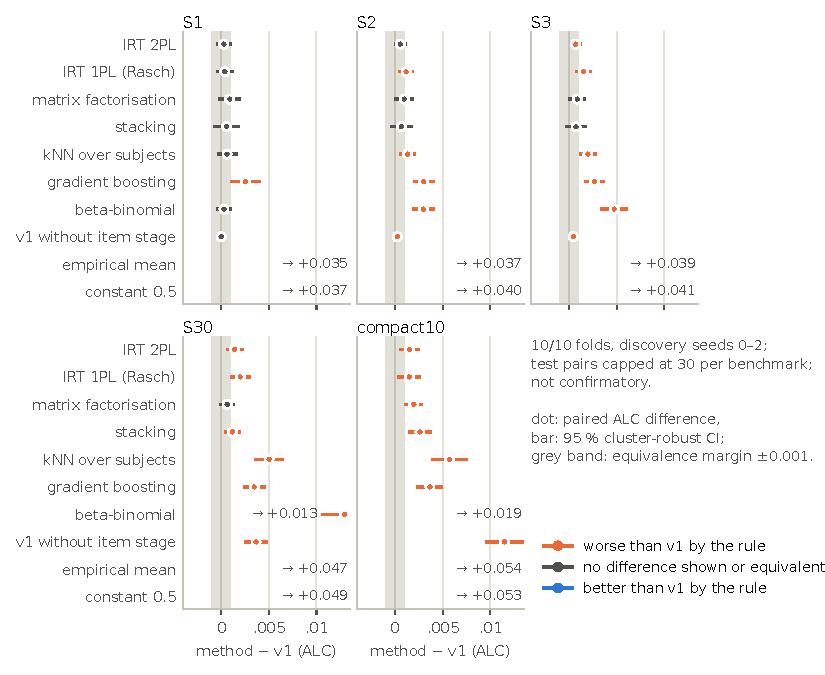
\includegraphics[width=\linewidth]{figA3_liga_forest.pdf}
  \caption{Method league (10 of 10 folds, discovery seeds): paired ALC difference method $-$ submitted
  model $\pm$ 95\% CI per regime (``v1'' on the axis = the submitted predictor along the v1 path, Appendix~\ref{app:prereg}), equivalence band $\pm 0.001$. Sources: Table~\ref{tab:figsources}.}
  \label{fig:league}
\end{figure}

\begin{figure}[H]
  \centering
  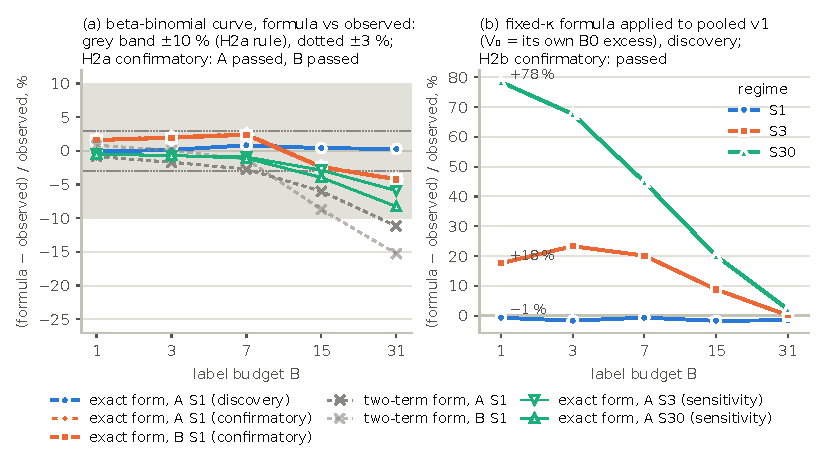
\includegraphics[width=\linewidth]{fig3_formel.pdf}
  \caption{Left: relative error of Eq.~\ref{eq:curve} against the observed \BB\ curve at $S = 1$, discovery (Design A)
  and confirmatory (Designs A and B), $\pm 10\%$ band; $S = 3$, $S = 30$ as sensitivity. Right: deviation of the fixed-$\kappa$
  form from the pooled submitted model (discovery; H2b). Sources: Table~\ref{tab:figsources}.}
  \label{fig:formula}
\end{figure}

\begin{figure}[H]
  \centering
  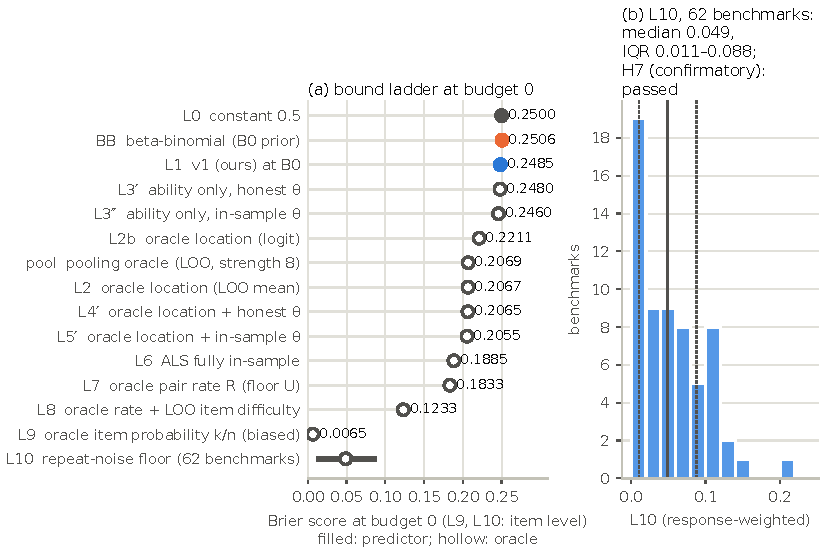
\includegraphics[width=\linewidth]{fig4_orakel_leiter.pdf}
  \caption{Bound ladder at budget 0 (Brier of oracles and predictors, discovery test pairs; Section~\ref{sec:theory}, A.5)
  and the per-benchmark noise floor L10 over the 62 benchmarks with $\ge 100$ repeated cells. Filled markers: predictors,
  hollow: oracles; the L9 and L10 rows are item-level. Sources: Table~\ref{tab:figsources}.}
  \label{fig:ladder}
\end{figure}

\begin{figure}[H]
  \centering
  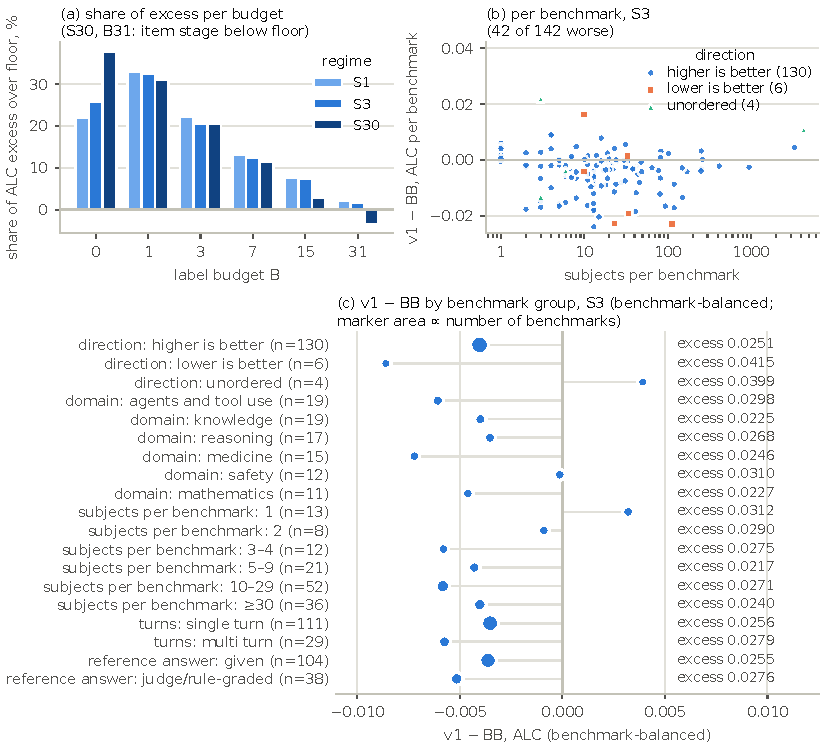
\includegraphics[width=\linewidth]{fig6_fehleranalyse.pdf}
  \caption{Error anatomy (discovery; (a) $S = 1, 3, 30$; (b), (c) $S = 3$). (a) Share of the excess over the pair-level floor per budget; (b)
  submitted $-$ \BB\ per benchmark against the number of subjects in the benchmark (42 of 142 benchmarks worse than
  \BB); (c) group means by polarity, domain, subjects per benchmark, turn type, reference answers (six largest domains; right: mean excess over the pair-level floor; polarity and turn type are missing for 2 of the 142 benchmarks).}
  \label{fig:errors}
\end{figure}

\begin{figure}[H]
  \centering
  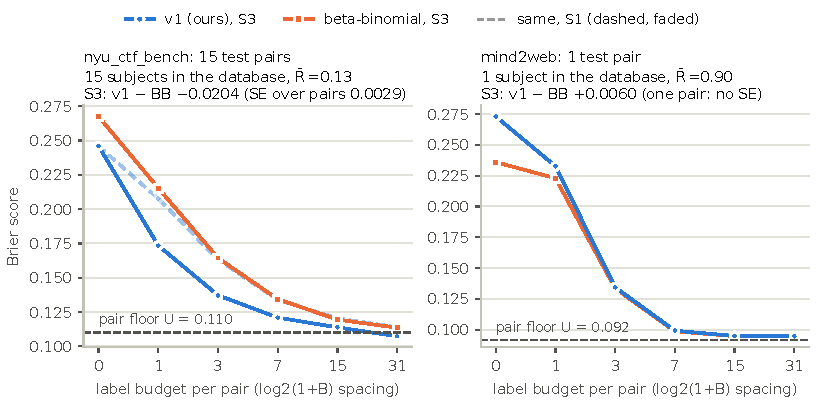
\includegraphics[width=\linewidth]{figA5_fallbeispiele.pdf}
  \caption{Two cases (discovery): NYU CTF Bench with one and three subjects sharing \texttt{labeled} (success), and
  Mind2Web, a single-subject benchmark (failure). Sources: Table~\ref{tab:figsources}.}
  \label{fig:cases}
\end{figure}

\begin{figure}[H]
  \centering
  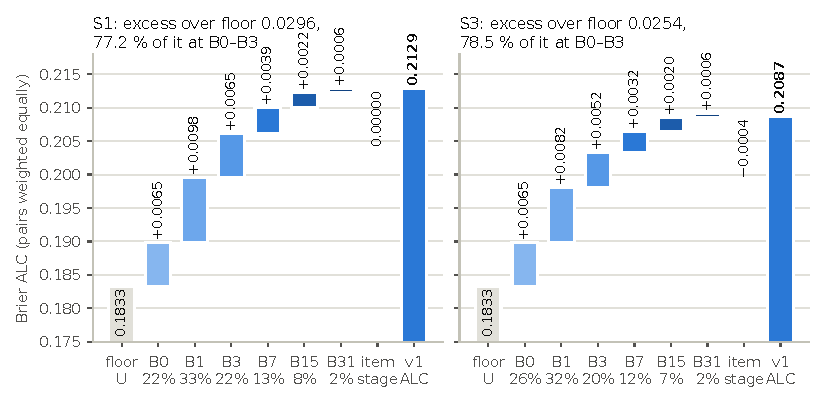
\includegraphics[width=\linewidth]{fig2_zerlegung.pdf}
  \caption{Decomposition of the ALC into pair floor and excess, per budget, $S = 1$ and $S = 3$ (discovery): floor $U$,
  ALC-weighted $(q-R)^2$ per budget (bar labels under the axis: share of the excess), item-stage gain, resulting ALC.
  Sources: Table~\ref{tab:figsources}.}
  \label{fig:waterfall}
\end{figure}

\begin{figure}[H]
  \centering
  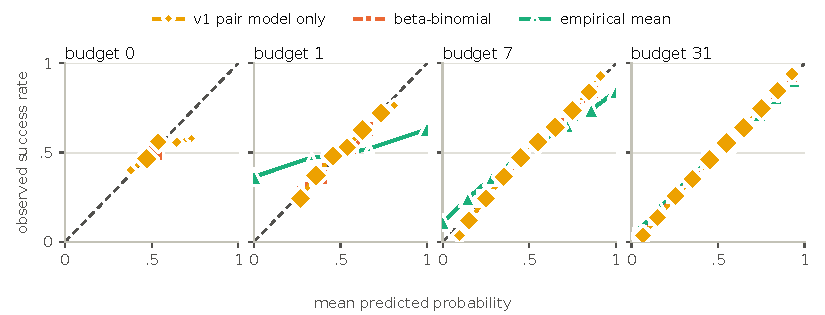
\includegraphics[width=\linewidth]{fig5_zuverlaessigkeit.pdf}
  \caption{Reliability diagrams at budgets 0, 1, 7 and 31 ($S = 3$, discovery) for the pair-level model, \BB\ and
  \EM; bins with fewer than 20 pair records hidden; marker area $\propto \sqrt{n}$. Item-stage reliability: not evaluated
  (no item-level reliability table in the result set). Sources: Table~\ref{tab:figsources}.}
  \label{fig:rel}
\end{figure}

\begin{figure}[H]
  \centering
  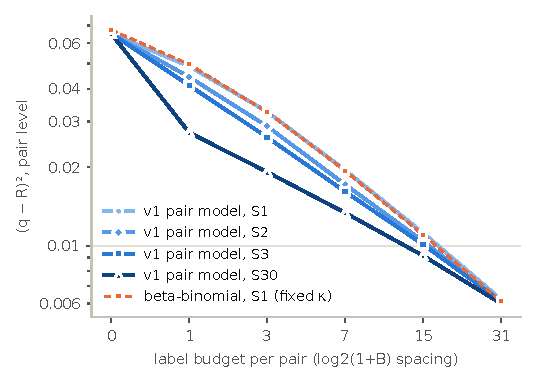
\includegraphics[width=0.65\linewidth]{figA1_v0_eff.pdf}
  \caption{Effective prior error $V_0(S, B)$ of the pooled pair-level model per regime and budget (discovery): the
  quantity that replaces the fixed $V_0$ of Eq.~\ref{eq:curve} for the submitted model. Sources: Table~\ref{tab:figsources}.}
  \label{fig:v0eff}
\end{figure}

\begin{figure}[H]
  \centering
  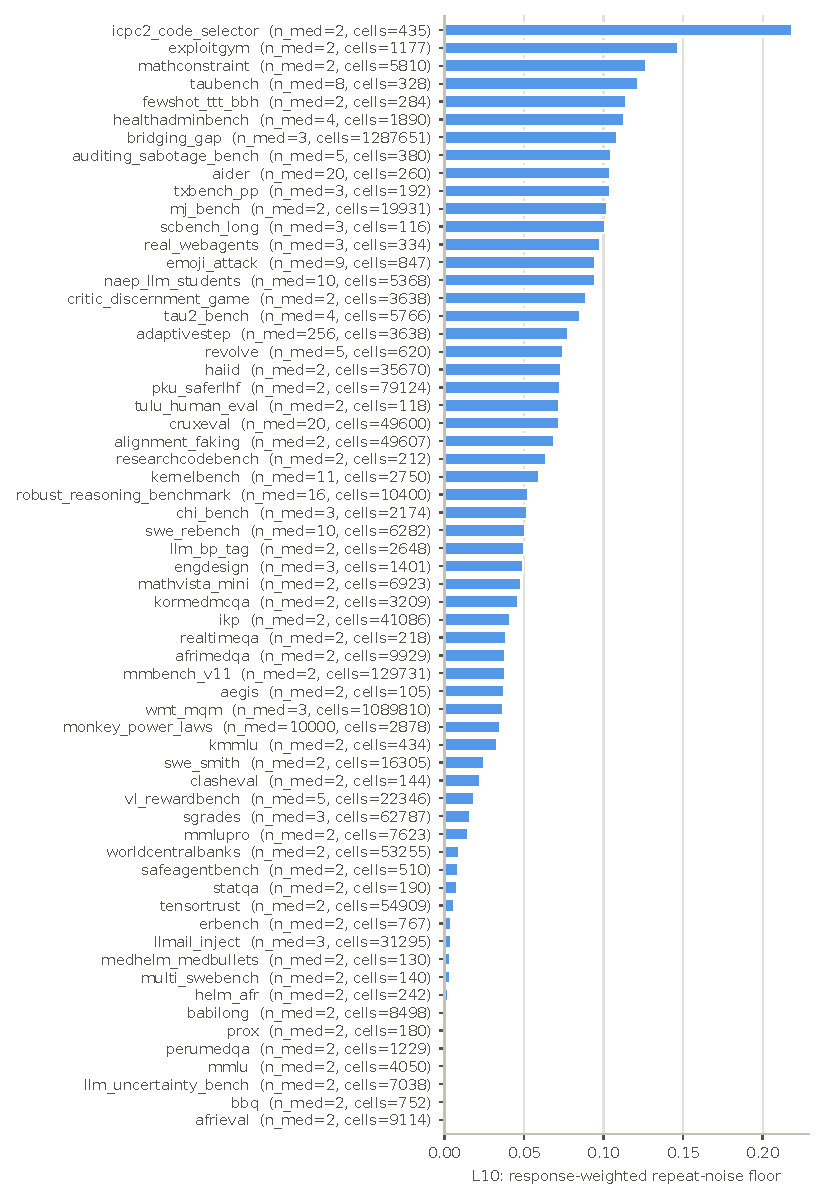
\includegraphics[width=\linewidth]{figA2_l10_je_benchmark.pdf}
  \caption{Response-noise floor L10 per benchmark (62 benchmarks with $\ge 100$ repeated cells), the curation metric
  released as \texttt{noise\_floor\_by\_benchmark.csv}; measurement-db revision \texttt{54074453}, second computation path
  (pandas) identical to the first (median exact; Table~\ref{tab:twopaths}). n\_med = median responses per repeated cell; cells = cells with $n \ge 2$. Sources: Table~\ref{tab:figsources}.}
  \label{fig:l10}
\end{figure}

\section{Data-quality audit: findings, lists, evidence packs}
\label{app:audit}

\textbf{Standard of evidence.} An observation is included only if (i) its key numbers were obtained by at least two
implementations with different code and, where possible, different data paths (Parquet footer statistics against the
column itself, Hugging Face originals (SHA-256 checked against the LFS object id) against cached copies, upstream
files fetched separately); (ii) where one exists, an external witness supports it (upstream file, publisher aggregate
or paper); (iii) harmless explanations (documented intent, another reading of the columns) were checked; (iv) two
further checks tried to refute it and failed. Where intent is plausible the observation is a question. Prior reports
were searched in the Hugging Face discussions, measurement-db pull requests \#1--\#7 and paiec\_baseline issues
\#1--\#3 (as of 2026-10-20); none covered these points except an overlap with one baseline issue on stale embeddings.
Everything was read-only; the proposed patches were checked with \texttt{git apply \dd check}, by re-implementing their
selection logic and, in the evidence packs, by regression tests that fail without the patch and pass with it.

\begin{table}[H]
  \caption{\raggedright The nine findings of the data-quality report, with the effect in the report's own wording. Revision
  \texttt{54074453}; checks run 2026-10-20. Source: Summary of the data-quality report sent to the organisers (not part of the repository; available on request); the public identifier-level lists are in \texttt{audit/}.}
  \label{tab:audit}
  \centering\scriptsize
  \begin{tabular}{@{}r>{\raggedright\arraybackslash}p{5.6cm}>{\raggedright\arraybackslash}p{2.6cm}>{\raggedright\arraybackslash}p{4.2cm}@{}}
    \toprule
    \# & Finding & Scope & Stated effect (report wording) \\
    \midrule
    1 & \texttt{tools/prepare\_data.py} sees 60 of 156 eligible graded benchmarks (\texttt{repo\_info().siblings} stops
        at 100,000 files); BLE \texttt{get\_benchmark} raises \texttt{KeyError}; embedding vectors keyed to pre-schema-3
        item IDs & baseline payload; 96 benchmarks missing & BLE and BLE-acquisition baselines run on a truncated corpus;
        scoring itself not affected \\
    2 & proofaug: an upstream archive is public although the curation record says it remains local and the upstream
        README asks not to distribute it (question) & 1 file, 68,666 bytes & none on measurements; concerns a third
        party's request \\
    3 & bird\_sql: 64 of 120 configurations graded 0 on all 360 questions; publisher's aggregate 5.6--40.6\% & 23,040
        grades (53\% of the benchmark) & wrong ability signal for these models in the training data \\
    4 & swebench\_live: 12 website-report subjects carry only successes (840 ones, no zeros); publisher rates 7--36\%
        (question) & 16 subjects (the 12 and those merged via website aliases) & 20\% of graded items carry only 1s; question whether the rule also applies in the
        test pool \\
    5 & Reasoning configuration not passed to the builder: configurations share one subject\_id; in ikp stored as trial
        1 and 2 & ikp: 30 subjects, 42,140 rows & $<1\%$ of eligible pairs; contradicts the subject definition and
        the meaning of \texttt{trial} \\
    6 & icpc2\_code\_selector: retrieval-free baseline run stored as trial 2 of gpt-4o on items showing retrieved
        candidates & 435 rows & small; wrong stimulus for these rows \\
    7 & Winogrande twins collapsed in published human translations: identical prompts, opposite gold answers
        (bridging\_gap, helm\_afr) & 117 upstream twin pairs (172 + 92 pairs in the database); 830 items & label noise in training data \\
    8 & 119 different models in 13 benchmarks receive identical competition input (\texttt{normalized\_name} null,
        label in no input field) & 25 groups & in devbench all subject information is lost \\
    9 & Documentation: card frozen at 255 folders; licence-field texts; 127 stale manifests; inventory rule wording;
        \texttt{test\_condition} contents; harness spellings; cross-benchmark item families & --- & mostly none; two
        questions concern the test pool \\
    \bottomrule
  \end{tabular}
\end{table}

{\raggedright\textbf{Lists and evidence packs} (folder \texttt{audit/} of the repository: identifiers, hashes and counts only; the
packs with record excerpts went to the organisers). Lists F1--F9g (row counts of the full lists sent to the organisers; the public \texttt{audit/csv/} omits F2, F3b and F9b, and F1, F9c, F9d and F9e each omit one row for a benchmark folder under a separate note, see \texttt{audit/README.md}): \texttt{F1\_baseline\_payload\_coverage.csv} (281
folders), \texttt{F2\_proofaug\_archive.csv} (1), \texttt{F3a\_bird\_sql\_configurations.csv} (120),
\texttt{F3b\_bird\_sql\_byte\_identical\_sql\_graded\_0.csv} (160), \texttt{F4\_swebench\_live\_subjects.csv} (65),
\texttt{F5a\_ikp\_merged\_configurations.csv} (30), \texttt{F5b\_reasoning\_setting\_only\_in\_label.csv} (218),
\texttt{F6\_icpc2\_gpt4o\_trials.csv} (435), \texttt{F7a}/\texttt{F7b} collapsed pairs (172, 92),
\texttt{F8\_identical\_input\_subject\_groups.csv} (119), \texttt{F9a}--\texttt{F9g} (26, 9, 127, 278, 176, 14, 45 rows).
Evidence packs (17): bird\_sql, swebench\_live, ikp, reasoning\_setting\_in\_label, icpc2\_code\_selector, bridging\_gap,
helm\_afr, identical\_subject\_inputs, measurement\_db\_embed, proofaug, docs\_9a--9g; each with \texttt{EVIDENCE.md},
affected-record lists, proposed corrections and an ``Ambiguities'' section. Patches (3, in the evidence-pack delivery; \texttt{audit/patches/} holds the earlier set of the data-quality report: full listing, optional skip of ungraded benchmarks, schema-3 columns): full folder listing without
\texttt{repo\_info}; schema-3 catalogue columns; matching published vectors to current item IDs (builds on the first);
each with an offline regression test and \texttt{verify\_patches.sh} against commit \texttt{cc88a959} and current
\texttt{main}. \textbf{Effect on this submission.} Findings 3 and 4 define the training exclusions of
Section~\ref{sec:data}; finding 8 is why the predictor groups labels by all eight fields; the other findings concern
baseline tooling, documentation or under 1\% of the scorable pairs, and the data were used as released. Audited
revisions and SHA-256 sums of every delivered file are in \texttt{SHA256SUMS} of the evidence-pack delivery sent to the organisers.\par}

\FloatBarrier
\section{Rerun: commands, hashes, two computation paths}
\label{app:rerun}

All commands run from the repository root with \texttt{PAIEC\_WORK} as the only path parameter and
\texttt{OMP\_NUM\_THREADS=1}; the Hugging Face token is read from \texttt{HF\_TOKEN} (the dataset is gated). Step 0
downloads \texttt{formatted\_tables} at revision \texttt{54074453} into a local base and is the only step that needs
network access.
\par\noindent\begin{minipage}{\linewidth}\small
\begin{verbatim}
export OMP_NUM_THREADS=1 PAIEC_WORK=./work   # and HF_TOKEN
make step0 daten    # 0: download_data.py, build_basis.py, daten.py (aggregation)
make tab-cv1 tab1   # 1: Design A phase 1+2 (seeds 0-2, fold seed 1234), CV tables
make fig            # 2: figures of the cross-validation
make smoke          # tests + hash check + fold 0 + comparison to reference, 1e-9
\end{verbatim}
\end{minipage}\par\medskip
The confirmatory runs (seeds 200--202), the method league and this report's figures and tables were produced with the
scripts in \texttt{konfirmation/}, \texttt{liga/} and \texttt{report/src/} (see their README files); they are not wired
into \texttt{make}, and their result files (\texttt{konfirmation/hypothesen\_tafel.json}, \texttt{liga/ergebnisse/},
\texttt{report/src/daten/}) are shipped in the repository.
Seeds: discovery 0, 1, 2 (fold assignment 1234, pair cap 30, cap seed 0); confirmatory 200, 201, 202 (fold assignment 200); league
inner tuning 100; bootstraps 200. Completion is checked mechanically (\texttt{status.json} reports 10 finished folds;
\texttt{auswertung.json} exists; the package check returns 0). Package: \texttt{\pkgfile} (\pkgbytes{} bytes; sha256
\texttt{\pkghashtex}; sha256 prefix of the embedded canonical state \texttt{\pkgstate}); a rebuild differs in the
embedded build time, so its checksum is not expected to match. Platform check: one formative Codabench evaluation of this package (submission 1008180; at most 1,000 subject--item pairs newly sampled from the hidden test data) returned Brier ALC 0.2056, inside the range of the offline replica (0.1968--0.2129 across regimes, Table~\ref{tab:main}); a single formative run has no standard error and was not used for any decision. Template: \texttt{neurips\_2026.sty}, workshop option
(\texttt{sglblindworkshop,final}). Hardware: 4 CPU cores, 16\,GiB RAM, no GPU; aggregation
46\,s, training 56\,s, one cross-validation design about 3 minutes (4 processes), league about 45 minutes per fold.

\begin{table}[H]
  \caption{\raggedright Two computation paths per core number (``match'' = agreement to the stated tolerance). Paths relative to the repository root;
  the primary audit scripts and the local result folders \texttt{cv\_REG*}, \texttt{cv\_V2K*} are not in the repository.}
  \label{tab:twopaths}
  \centering\scriptsize
  \begin{tabular}{@{}>{\raggedright\arraybackslash}p{3.5cm}>{\raggedright\arraybackslash}p{3.3cm}>{\raggedright\arraybackslash}p{3.2cm}>{\raggedright\arraybackslash}p{2.4cm}@{}}
    \toprule
    number & path A & path B & match \\
    \midrule
    L10 median 0.0488 (62 benchmarks) & \texttt{report/\allowbreak src/\allowbreak analyse/\allowbreak wiederholung.py} on \texttt{agg.parquet}, closed-form estimator &
      \texttt{curation/\allowbreak wiederholung\_b.py}, pandas on raw responses, \texttt{var(ddof=1)} & exact (summaries $\le 5\times10^{-16}$ rel.) \\
    Formula values Eq.~\ref{eq:curve} & \texttt{theorie/\allowbreak alc\_law.py} (standard library) & \texttt{report/\allowbreak src/\allowbreak plots\_v2.py} and \texttt{tabellen\_v2.py}
      re-implementation from JSON moments & identical (log: \texttt{formel\_check.log}) \\
    Split-term approximation 0.2130 ALC & \texttt{report/\allowbreak src/\allowbreak analyse/\allowbreak split.py} (discovery) & \texttt{theorie/\allowbreak alc\_law.py \dd split quadrat} & $10^{-6}$ \\
    EM and BB baselines & \texttt{modell/baselines.py} (CV harness) & league harness \texttt{liga/\allowbreak liga\_methoden.py} &
      max $|\Delta q| = 0$ \\
    v1 path vs.\ submitted v2.0-core path & \texttt{cv\_REG1}/\texttt{cv\_REG2} (v1) & \texttt{cv\_V2K1}/\texttt{cv\_V2K2}
      (v2.0-core) & $|\Delta q| = 0$ on 1,079,568 and 1,214,136 records (phase 2: outside nested Platt stages) \\
    L9 item oracle 0.0065 & \texttt{report/\allowbreak src/\allowbreak analyse/\allowbreak leiter.py} (test pairs, pair-weighted) & \texttt{curation/\allowbreak wiederholung\_b.py}
      (\texttt{l9\_abgleich}) & 0.00649 vs 0.00652 \\
    Audit findings 1, 3--9 & primary scripts (\texttt{check1}--\texttt{check6}) & second implementation per finding
      (different code and data path, same author workflow) & key numbers equal (data-quality report) \\
    \bottomrule
  \end{tabular}
\end{table}

% erzeugt von plots_v2.py (nicht von Hand aendern)
\begin{table}[H]
  \caption{\raggedright Data files read by the figure script for each figure (paths relative to the repository root; \texttt{daten/} = \texttt{report/src/daten/}).}
  \label{tab:figsources}
  \centering\scriptsize
  \begin{tabular}{@{}l>{\raggedright\arraybackslash}p{0.86\linewidth}@{}}
    \toprule
    figure & files \\
    \midrule
    \ref{fig:map} & \texttt{modell/\allowbreak{}ergebnisse/\allowbreak{}cv\_\allowbreak{}A\_\allowbreak{}p2\_\allowbreak{}S1-S2-S3-S30-kompakt10/\allowbreak{}auswertung.json (tabelle\_\allowbreak{}alle, vergleiche); floors: daten/\allowbreak{}beobachtung\_\allowbreak{}discovery.json (U\_\allowbreak{}E), daten/\allowbreak{}D\_\allowbreak{}exakt.json, daten/\allowbreak{}leiter.json (L8), curation/\allowbreak{}wiederholung\_\allowbreak{}b.json (L10); formula: theorie/\allowbreak{}alc\_\allowbreak{}law.py.} \\
    \ref{fig:league} & \texttt{liga/\allowbreak{}ergebnisse/\allowbreak{}vergleich\_\allowbreak{}gepaart.csv (mittel, ki95\_\allowbreak{}unten, ki95\_\allowbreak{}oben, urteil), liga/\allowbreak{}ergebnisse/\allowbreak{}meta.json (falten, saaten).} \\
    \ref{fig:formula} & \texttt{(a) daten/\allowbreak{}beobachtung\_\allowbreak{}discovery.json + daten/\allowbreak{}D\_\allowbreak{}exakt.json via theorie/\allowbreak{}alc\_\allowbreak{}law.py; konfirmation/\allowbreak{}hypothesen\_\allowbreak{}tafel.json (H2a, teile.A.S1, teile.B.S1). (b) daten/\allowbreak{}beobachtung\_\allowbreak{}discovery.json (S1/\allowbreak{}S3/\allowbreak{}S30 hier\_\allowbreak{}item).} \\
    \ref{fig:ladder} & \texttt{daten/\allowbreak{}leiter.json (leiter\_\allowbreak{}B0), daten/\allowbreak{}leiter\_\allowbreak{}ergaenzung.json (L2b, L3', L3'', L4', L5'), modell/\allowbreak{}ergebnisse/\allowbreak{}cv\_\allowbreak{}A\_\allowbreak{}p2\_\allowbreak{}S1-S2-S3-S30-kompakt10/\allowbreak{}auswertung.json (BB B0), daten/\allowbreak{}e3.json (pooling oracle S1 B0), curation/\allowbreak{}wiederholung\_\allowbreak{}b.json + curation/\allowbreak{}noise\_\allowbreak{}floor\_\allowbreak{}by\_\allowbreak{}benchmark.csv (L10). Design A, discovery (seeds 0–2).} \\
    \ref{fig:errors} & \texttt{daten/\allowbreak{}verlust.json (alc\_\allowbreak{}anteil\_\allowbreak{}*, gruppe\_\allowbreak{}*, n\_\allowbreak{}benchmarks\_\allowbreak{}schlechter\_\allowbreak{}als\_\allowbreak{}bb), daten/\allowbreak{}je\_\allowbreak{}benchmark.csv (gewinn\_\allowbreak{}vs\_\allowbreak{}bb, n\_\allowbreak{}subjects, direction).} \\
    \ref{fig:cases} & \texttt{curation/\allowbreak{}fallbeispiele.json (brier\_\allowbreak{}je\_\allowbreak{}budget, floor\_\allowbreak{}R(1-R), diff\_\allowbreak{}hier\_\allowbreak{}item\_\allowbreak{}minus\_\allowbreak{}bb\_\allowbreak{}alc, n\_\allowbreak{}subjects\_\allowbreak{}db).} \\
    \ref{fig:waterfall} & \texttt{daten/\allowbreak{}verlust.json (alc\_\allowbreak{}anteil\_\allowbreak{}S1/\allowbreak{}S3, budget\_\allowbreak{}hier\_\allowbreak{}item: sq, itemg, floor); weights 0.1/\allowbreak{}0.2/\allowbreak{}0.2/\allowbreak{}0.2/\allowbreak{}0.2/\allowbreak{}0.1.} \\
    \ref{fig:rel} & \texttt{modell/\allowbreak{}ergebnisse/\allowbreak{}cv\_\allowbreak{}A\_\allowbreak{}p2/\allowbreak{}zuverlaessigkeit.csv (praediktor, budget, bin, n, q\_\allowbreak{}mittel, R\_\allowbreak{}mittel); regime from modell/\allowbreak{}ergebnisse/\allowbreak{}cv\_\allowbreak{}A\_\allowbreak{}p2/\allowbreak{}auswertung.json primaer\_\allowbreak{}S.} \\
    \ref{fig:v0eff} & \texttt{daten/\allowbreak{}verlust.json (pooling\_\allowbreak{}sq), daten/\allowbreak{}beobachtung\_\allowbreak{}discovery.json (S1/\allowbreak{}beta\_\allowbreak{}binomial).} \\
    \ref{fig:l10} & \texttt{curation/\allowbreak{}noise\_\allowbreak{}floor\_\allowbreak{}by\_\allowbreak{}benchmark.csv (L10\_\allowbreak{}response\_\allowbreak{}weighted, cells\_\allowbreak{}rep, n\_\allowbreak{}median\_\allowbreak{}rep).} \\
    \bottomrule
  \end{tabular}
\end{table}


\section{Reference check}
\label{app:bib}
% erzeugt von bericht-v2/baue_refs.py (nur zitierte Schluessel) -- nicht von Hand aendern
\begin{table}[H]
  \caption{Reference check. Of the 32 references cited in this report, the bibliographic record (authors, title, year, venue) was checked against the arXiv record or the DOI record, or the page or repository was accessed, on 20--21 October 2026. The checks were carried out by AI agents under the author's direction (Section ``Use of AI assistants'') and cover the record, not the full text. A venue given ``per arXiv comment'' is the one stated in the arXiv record and was not checked at the publisher.}
  \label{tab:bibcheck}
  \centering\scriptsize
  \setlength{\tabcolsep}{3pt}
  \begin{tabular}{@{}>{\raggedright\arraybackslash}p{3.3cm}>{\raggedright\arraybackslash}p{3.1cm}@{\hspace{10pt}}>{\raggedright\arraybackslash}p{3.3cm}>{\raggedright\arraybackslash}p{3.1cm}@{}}
    \toprule
    key & check & key & check \\
    \midrule
    \citet{brier1950} & DOI record checked & \citet{morris1983peb} & DOI record checked \\
    \citet{cameron2015cluster} & DOI record checked & \citet{murphy1973partition} & DOI record checked \\
    \citet{efron1975stein} & DOI record checked & \citet{northcutt2021pervasive} & arXiv record checked \\
    \citet{fox2010bayesianirt} & DOI record checked & \citet{owen2024predictable} & arXiv record checked \\
    \citet{gema2024mmlu} & arXiv record + DOI record checked & \citet{pacchiardi2024hundred} & arXiv record checked \\
    \citet{gneiting2007proper} & DOI record checked & \citet{platt1999probabilistic} & DOI record of the edited volume checked \\
    \citet{guyon2011alc} & page or repository accessed & \citet{ruan2024observational} & arXiv record checked \\
    \citet{kipnis2024metabench} & arXiv record checked & \citet{rubin1976} & DOI record checked \\
    \citet{koren2009mf} & DOI record checked & \citet{sawade2010activerisk} & page or repository accessed \\
    \citet{kossen2021activetesting} & arXiv record checked & \citet{mdb2026} & page or repository accessed \\
    \citet{lalor2016irt} & DOI record checked & \citet{paiec2026} & page or repository accessed \\
    \citet{lord1980irt} & DOI record checked & \citet{paiecbase2026} & page or repository accessed \\
    \citet{mackay1992evidence} & DOI record checked & \citet{truong2025amortized} & arXiv record + proceedings page checked \\
    \citet{madaan2024variance} & arXiv record checked & \citet{vivek2023anchor} & arXiv record + DOI record checked \\
    \citet{polo2024tiny} & arXiv record + proceedings page checked & \citet{wolpert1992} & DOI record checked \\
    \citet{miller2024errorbars} & arXiv record checked & \citet{zhou2025adele} & arXiv record checked \\
    \bottomrule
  \end{tabular}
\end{table}


\section{Exploratory work, not completed, not part of the submission}
\label{app:explore}

\textbf{Stratum stage.} A third level between pair and item (strata of items by visible metadata keys, with the
item offset residualised on the stratum) was implemented with 22 unit tests (bit-identical to the submitted model
without item features; a deliberate ``no shrinkage'' failure case triggered). A pilot on one fold ran; the full
cross-validation was aborted when the compute budget was reallocated, so no gate decision was possible and no result
is reported. \textbf{Text-based item prior.} Item texts of 123 benchmarks (114,030 items) were fetched by range
requests and embedded with a small sentence encoder on CPU; five hypotheses (within-benchmark $R^2$ of a ridge on
embeddings for item difficulty, cross-benchmark transfer, benchmark location from mean embeddings, ALC effect of a
text prior at three subjects between $-0.006$ and $-0.001$, runtime limits) were fixed before any evaluation. No
evaluation was run before the freeze; nothing is reported, and the submitted predictor uses no text. \textbf{Acquisition
function.} A coverage-based acquisition policy for the platform's \texttt{labeling.py} interface (\texttt{akquise/politiken.py}; Appendix~\ref{app:theory}, A.7) was implemented with a simulator of
the platform's streaming acquisition (sha256-uniform replica; lemma 1 checked bit-identically on 15,000 candidates;
failure cases: broken \texttt{labeled} triggers the fallback, a leaked simulator triggers the leak assertion). A pilot on
fold 0 fixed the operating characteristic (minimal detectable effect in compact10 0.00034 with 3 seeds); the full run
over regimes, orderings and split designs was aborted, so the gate was not evaluated and the platform's random
acquisition is used. The pilot numbers in Table~\ref{tab:protocol} are labelled as such.

\end{document}
